\documentclass[mathserif,compress]{beamer}\usepackage{graphicx, color}
%% maxwidth is the original width if it is less than linewidth
%% otherwise use linewidth (to make sure the graphics do not exceed the margin)
\makeatletter
\def\maxwidth{ %
  \ifdim\Gin@nat@width>\linewidth
    \linewidth
  \else
    \Gin@nat@width
  \fi
}
\makeatother

\definecolor{fgcolor}{rgb}{0.2, 0.2, 0.2}
\newcommand{\hlnumber}[1]{\textcolor[rgb]{0,0,0}{#1}}%
\newcommand{\hlfunctioncall}[1]{\textcolor[rgb]{0.501960784313725,0,0.329411764705882}{\textbf{#1}}}%
\newcommand{\hlstring}[1]{\textcolor[rgb]{0.6,0.6,1}{#1}}%
\newcommand{\hlkeyword}[1]{\textcolor[rgb]{0,0,0}{\textbf{#1}}}%
\newcommand{\hlargument}[1]{\textcolor[rgb]{0.690196078431373,0.250980392156863,0.0196078431372549}{#1}}%
\newcommand{\hlcomment}[1]{\textcolor[rgb]{0.180392156862745,0.6,0.341176470588235}{#1}}%
\newcommand{\hlroxygencomment}[1]{\textcolor[rgb]{0.43921568627451,0.47843137254902,0.701960784313725}{#1}}%
\newcommand{\hlformalargs}[1]{\textcolor[rgb]{0.690196078431373,0.250980392156863,0.0196078431372549}{#1}}%
\newcommand{\hleqformalargs}[1]{\textcolor[rgb]{0.690196078431373,0.250980392156863,0.0196078431372549}{#1}}%
\newcommand{\hlassignement}[1]{\textcolor[rgb]{0,0,0}{\textbf{#1}}}%
\newcommand{\hlpackage}[1]{\textcolor[rgb]{0.588235294117647,0.709803921568627,0.145098039215686}{#1}}%
\newcommand{\hlslot}[1]{\textit{#1}}%
\newcommand{\hlsymbol}[1]{\textcolor[rgb]{0,0,0}{#1}}%
\newcommand{\hlprompt}[1]{\textcolor[rgb]{0.2,0.2,0.2}{#1}}%

\usepackage{framed}
\makeatletter
\newenvironment{kframe}{%
 \def\at@end@of@kframe{}%
 \ifinner\ifhmode%
  \def\at@end@of@kframe{\end{minipage}}%
  \begin{minipage}{\columnwidth}%
 \fi\fi%
 \def\FrameCommand##1{\hskip\@totalleftmargin \hskip-\fboxsep
 \colorbox{shadecolor}{##1}\hskip-\fboxsep
     % There is no \\@totalrightmargin, so:
     \hskip-\linewidth \hskip-\@totalleftmargin \hskip\columnwidth}%
 \MakeFramed {\advance\hsize-\width
   \@totalleftmargin\z@ \linewidth\hsize
   \@setminipage}}%
 {\par\unskip\endMakeFramed%
 \at@end@of@kframe}
\makeatother

\definecolor{shadecolor}{rgb}{.97, .97, .97}
\definecolor{messagecolor}{rgb}{0, 0, 0}
\definecolor{warningcolor}{rgb}{1, 0, 1}
\definecolor{errorcolor}{rgb}{1, 0, 0}
\newenvironment{knitrout}{}{} % an empty environment to be redefined in TeX

\usepackage{alltt} 
\usepackage{beamerthemeDresden} 
\usepackage[english]{babel}
\usepackage{amsmath,amssymb}
\usepackage[latin1]{inputenc}
\usepackage{palatino}
\usepackage{graphicx}
\usepackage{subfigure}
\usepackage{pgf}
\usepackage{relsize}
\def\beq{\begin{equation}}
\def\eeq{\end{equation}}
\def\bit{\begin{itemize}}
\def\eit{\end{itemize}}
\def\bdm{\begin{displaymath}}
\def\edm{\end{displaymath}}
\def\ben{\begin{enumerate}}
\def\een{\end{enumerate}}
\def\bc{\mathbf{c}}
\def\bh{\mathbf{h}}
\def\br{\mathbf{r}}
\def\bs{\mathbf{s}}
\def\bu{\mathbf{u}}
\def\bw{\mathbf{w}}
\def\bx{\mathbf{x}}
\def\by{\mathbf{y}}
\def\bz{\mathbf{z}}
\def\bA{\mathbf{A}}
\def\bD{\mathbf{D}}
\def\bG{\mathbf{G}}
\def\bI{\mathbf{I}}
\def\bQ{\mathbf{Q}}
\def\bR{\mathbf{R}}
\def\bS{\mathbf{S}}
\def\bV{\mathbf{V}}
\def\bW{\mathbf{W}}
\def\bX{\mathbf{X}}
\def\bY{\mathbf{Y}}
\def\bZ{\mathbf{Z}}
\def\cB{\mathcal{B}}
\def\cF{\mathcal{F}}
\def\cI{\mathcal{I}}
\def\cK{\mathcal{K}}
\def\cU{\mathcal{U}}
\def\bbeta{\mbox{\boldmath $\beta$}}
\def\bepsilon{\mbox{\boldmath $\epsilon$}}
\def\bdelta{\mbox{\boldmath $\delta$}}
\def\bgamma{\mbox{\boldmath $\gamma$}}
\def\bldeta{\mbox{\boldmath $\eta$}}
\def\bphi{\mbox{\boldmath $\phi$}}
\def\bkappa{\mbox{\boldmath $\kappa$}}
\def\blambda{\mbox{\boldmath $\lambda$}}
\def\bmu{\mbox{\boldmath $\mu$}}
\def\bnu{\mbox{\boldmath $\nu$}}
\def\btheta{\mbox{\boldmath $\theta$}}
\def\brho{\mbox{\boldmath $\rho$}}
\def\bDelta{\mbox{\boldmath $\Delta$}}
\def\bLambda{\mbox{\boldmath $\Lambda$}}
\def\bSigma{\mbox{\boldmath $\Sigma$}}
\def\var{\textrm{var}}
\def\cov{\textrm{cov}}
\def\log{\textrm{log}}
\def\median{\textrm{median}}
\def\argmin{\textrm{arg min }}
\def\bzero{\mathbf{0}}
\def\bone{\mathbf{1}}
\def\Poi{\textrm{Poi}}
\def\Unif{\textrm{Unif}}
\def\upp{^\prime}
\def\upi{^{-1}}
\newcommand{\cye}[1]{\color{yellow!70!black}#1}
\newcommand{\cre}[1]{\color{red!70!black}#1}
\newcommand{\cbl}[1]{\color{blue!70!black}#1}
\newcommand{\cgr}[1]{\color{green!70!black}#1}
\IfFileExists{upquote.sty}{\usepackage{upquote}}{}
\begin{document}


\title[]{Introduction to Spatial Statistics}

\author[Jay M. Ver Hoef]{Jay Ver Hoef} 

\institute[NOAA National Marine Mammal Lab]
{
	\normalsize National Marine Mammal Lab \\
	NOAA Fisheries \\
	International Arctic Research Center \\
	Fairbanks, Alaska, USA\\
	\vspace{0.1cm}
}
\date[05/17/13]{}
 
\maketitle
 
% very important to use option [fragile] for frames containing code output!
%-------------------------------------------------------------------------------
%                        OUTLINE
%-------------------------------------------------------------------------------

\section{Introduction}
\subsection{}
\begin{frame} [fragile]
\frametitle{Outline}
   
	\begin{tabular} {p{3.8cm} p{5.8cm}}

		\begin{center}
		\vspace{-.3cm}
		\bit
			\item Introduction     
			\item Autocorrelation         
			\item Types of Spatial Data    
			\item Prediction    
			\item Regression 
			\item Design of Experiments 
			\item Sampling 
			\item Summary
		\eit
	\end{center}
 &
		\vspace{-1.4cm}






\begin{knitrout}\tiny
\definecolor{shadecolor}{rgb}{0.969, 0.969, 0.969}\color{fgcolor}

{\centering 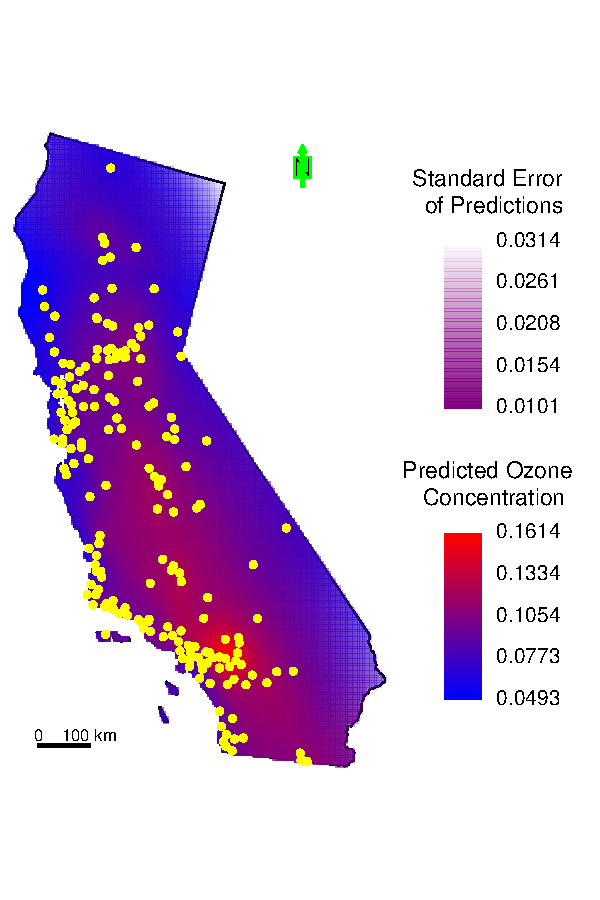
\includegraphics[width=\maxwidth]{figure/CA-predMap} 

}



\end{knitrout}

	\end{tabular}

\end{frame}

%-------------------------------------------------------------------------------
%                        What Are Statistics?
%-------------------------------------------------------------------------------

\begin{frame} 
\frametitle{What are Statistics?}
     
	\begin{tabular} {p{4.5cm} p{4.5cm}}

			{\bdm
				\bar{z} = \frac{1}{n}\sum_{i = 1}^n z_i 
			\edm} &
			\vspace{.2cm}
			{A statistic is a function of data} 
		  \\
		
		\begin{center}
		  \vspace{-.5cm}
			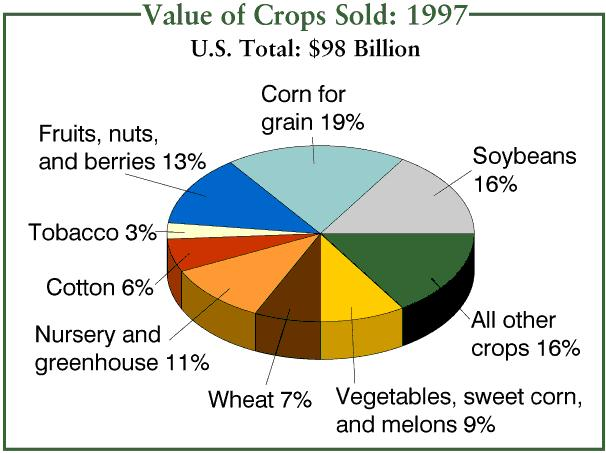
\includegraphics[width=4.0cm]{figure/pieChart.jpeg} 
		  \vspace{.5cm}
		\end{center} &
		\begin{center}
			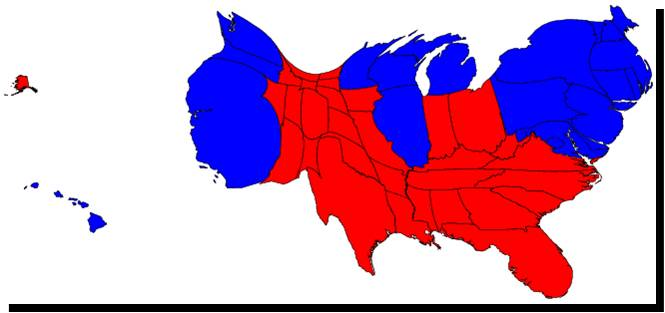
\includegraphics[width=4.4cm]{figure/voteMap.jpg} 
		  \vspace{.5cm}
		\end{center} 
		

	\end{tabular}

\end{frame}

%-------------------------------------------------------------------------------
%                        What Are Statistics?
%-------------------------------------------------------------------------------

\begin{frame} 
\frametitle{Statistical Models and Inference}
     
		\begin{center}
		  \vspace{-.5cm}
			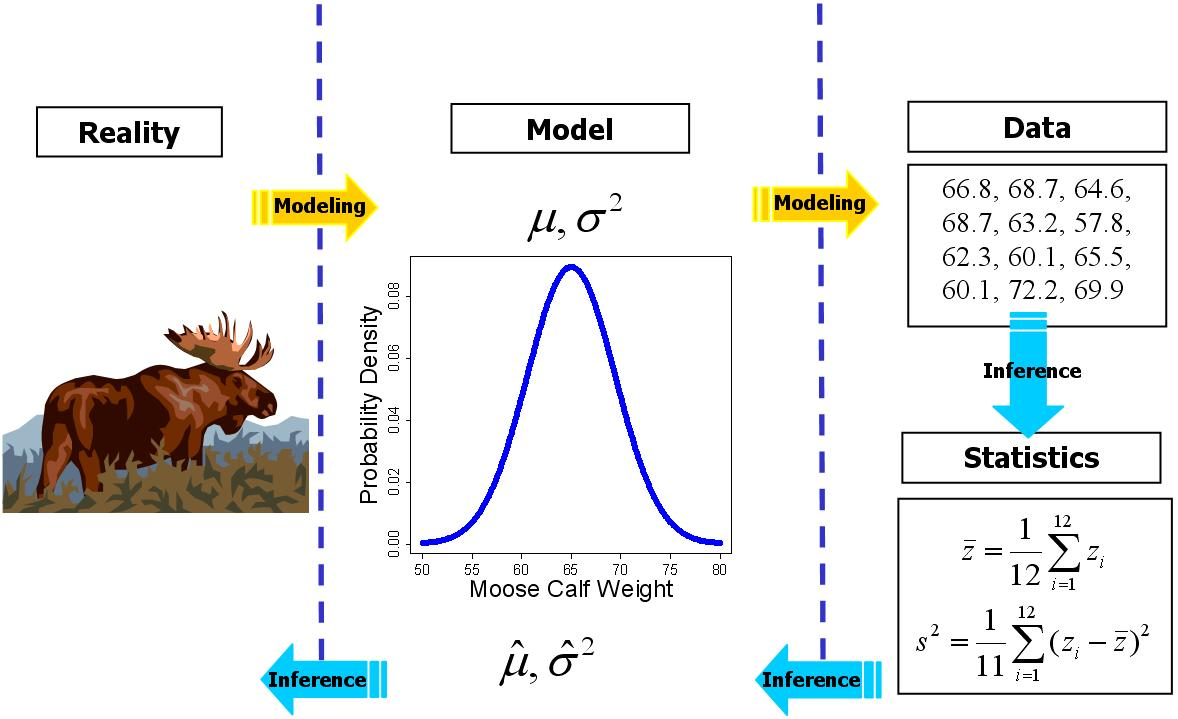
\includegraphics[width=10.4cm]{figure/statModInfer.jpeg} 
		\end{center} 
\end{frame}
  
%-------------------------------------------------------------------------------
%                        What is a Model?
%-------------------------------------------------------------------------------

\begin{frame} 
\frametitle{What is a Model?}
     
	\begin{tabular} {p{4.5cm} p{4.5cm}}
		
		\begin{center}
			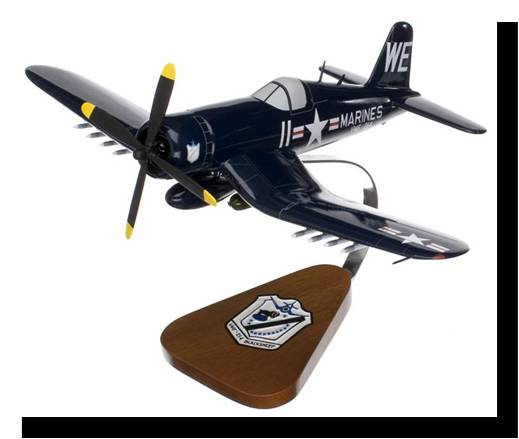
\includegraphics[width=4.0cm]{figure/airplane1.jpg} 
		\end{center} &
		\begin{center}
			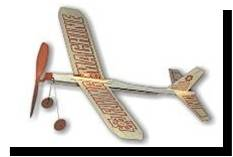
\includegraphics[width=4.0cm]{figure/airplane2.jpg} 
		\end{center} \\

	\bit
		\item{{\color{green!70!black}What does it look like?}} 
		\item{{\color{green!70!black}Structural}} 
	\eit &
	\bit
		\item{{\color{blue!70!black}How does it work?}}
		\item{{\color{blue!70!black}Functional}}
	\eit

	\end{tabular}

\end{frame}

%-------------------------------------------------------------------------------
%                        What Are Statistics?
%-------------------------------------------------------------------------------

\begin{frame} 
\frametitle{Spatial Statistical Models and Inference}
     
		\begin{center}
		  \vspace{-.5cm}
			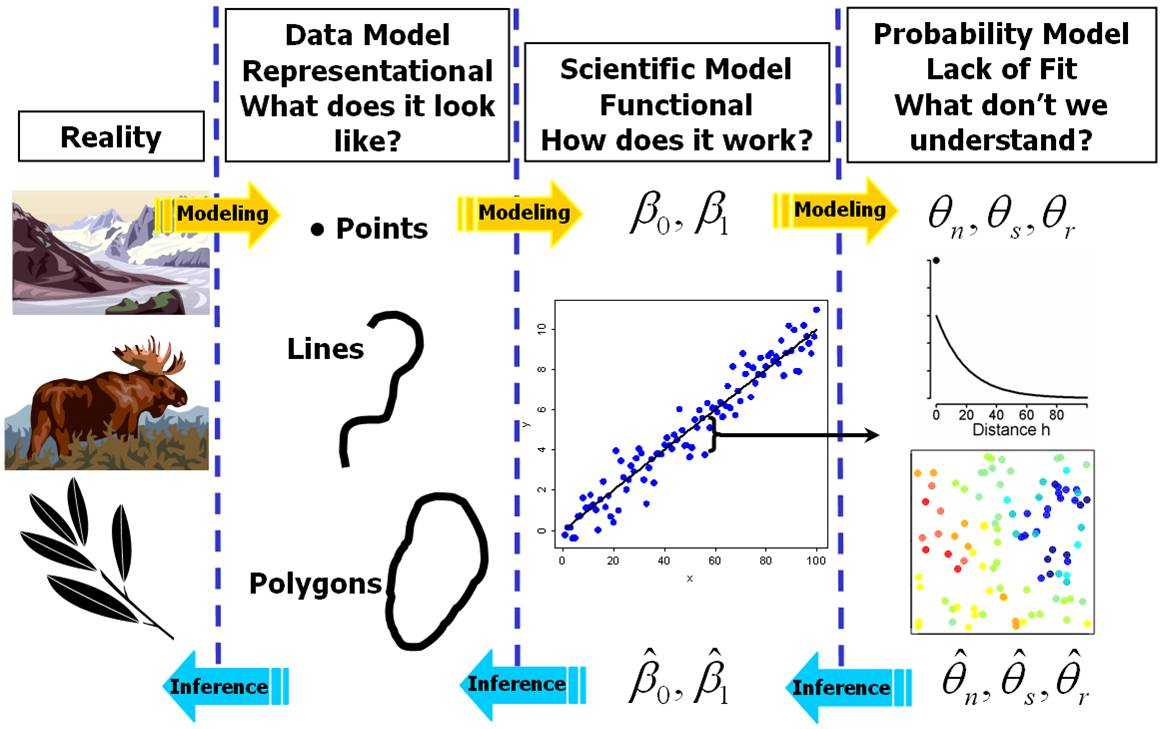
\includegraphics[width=10.4cm]{figure/repSpModInfer.jpg} 
		\end{center} 
\end{frame}

%-------------------------------------------------------------------------------
%                         Linear Model
%-------------------------------------------------------------------------------

\begin{frame} 
\frametitle{Spatial Linear Model}
     
	\begin{tabular} {p{4.5cm} p{.5cm} p{4.5cm}}
		\vspace{-.2cm} \[ z_i \] & \vspace{.1cm}  = & \vspace{-.6cm}
			\[\beta_0 + x_{1,i}\beta_1 + x_{2,i}\beta_2 + \ldots + \epsilon_i \] \\
		\vspace{-.6cm} \[ z_{j,k,i} \] & \vspace{-.3cm} = &  \vspace{-1cm}
			\[\beta_0 + \tau_{j} + \delta_{k} + (\tau\delta)_{j,k} + 
			\ldots + \epsilon_{j,k,i} 	\] \\
		\vspace{-.6cm} \[
			\left(\begin{array}{c}	
					\bz_{\textrm{observed}} \\
					{\color{green!70!black} \bz_{\textrm{unobserved}}}
				\end{array} \right) 
		\] & \vspace{-.2cm} = & 
		\vspace{-.9cm} \[\bX{\color{yellow!70!black}\bbeta} + 
			\bepsilon, \ \var(\bepsilon) = \bSigma({\color{red!70!black}\btheta}) \] \\
		\bit
			\item{{\color{green!70!black}Point Prediction}} 
			\item{{\color{green!70!black}Block Prediction}} 
			\item{{\color{green!70!black}Sampling}} 
		\eit & &
		\bit
			\item{{\color{yellow!70!black}Regression}} 
			\item{{\color{yellow!70!black}Design of Experiments}}
		\eit
	\end{tabular}

\end{frame}

%-------------------------------------------------------------------------------
%                        What Are Statistics?
%-------------------------------------------------------------------------------

\begin{frame} 
\frametitle{Covariance Matrix in Spatial Linear Models}
    
	\vspace{.2cm}
	\begin{tabular} {p{5cm} p{4cm}}
		\multicolumn{2}{c}{Reduce the number of parameters in the probability model} \\
		 \multicolumn{2}{c}{by using spatial relationships} \\
		\vspace{-.5cm}
		\begin{equation*} 
			 \bSigma = \left( \begin{array}{cccc}
				\sigma_{1,1} & \sigma_{1,2} & \cdots & \sigma_{1,n} \\
				\sigma_{2,1} & \sigma_{2,2} & \cdots & \sigma_{2,n} \\
				\vdots & \vdots & \cdots & \vdots \\
				\sigma_{n,1} & \sigma_{n,2} & \cdots & \sigma_{n,n} 
			\end{array} \right)
		\end{equation*} &

 		\vspace{-.1cm}
\begin{knitrout}\tiny
\definecolor{shadecolor}{rgb}{0.969, 0.969, 0.969}\color{fgcolor}

{\centering 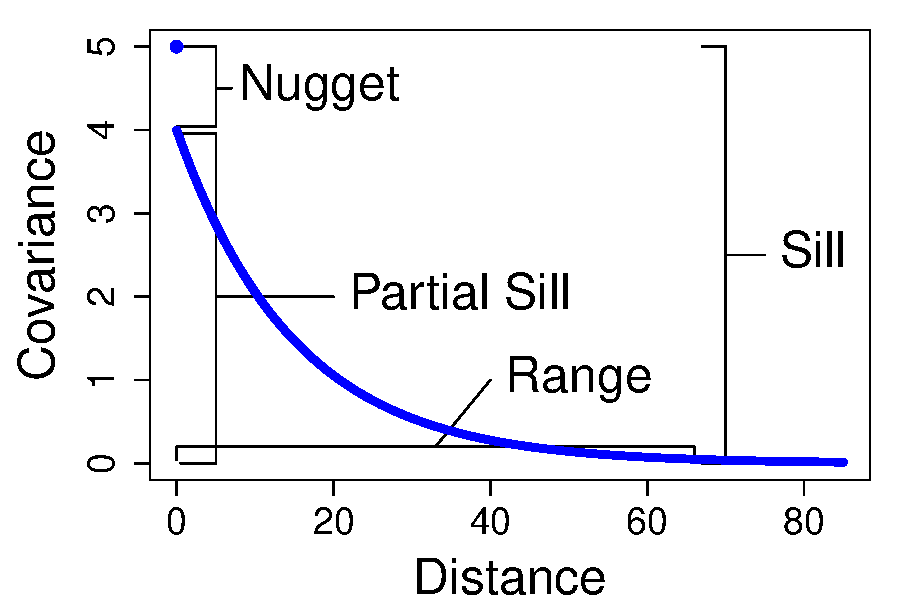
\includegraphics[width=\maxwidth]{figure/autCovGraph} 

}



\end{knitrout}

 		\\
		\vspace{-.8cm}
		\hspace{1cm} 
		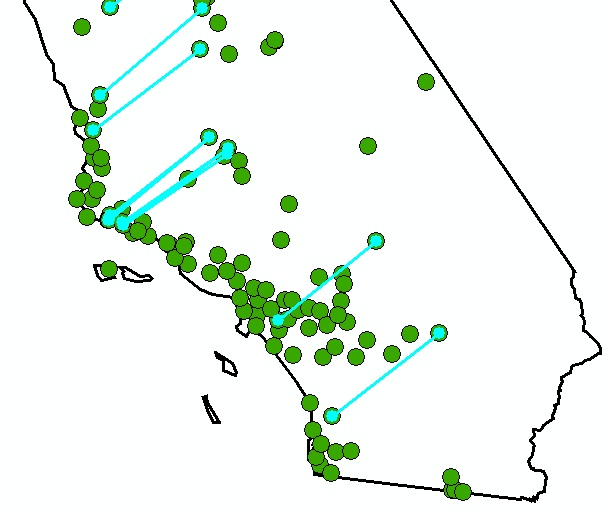
\includegraphics[width=2.8cm]{figure/sCalOzoneDistances1.jpg} &
		\vspace{-.8cm}
		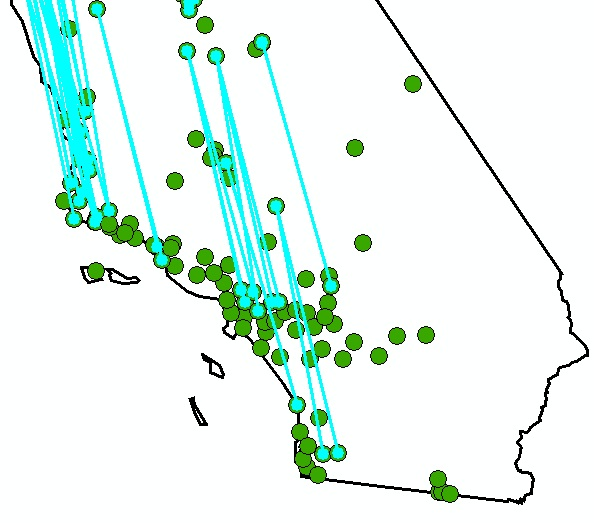
\includegraphics[width=2.8cm]{figure/sCalOzoneDistances2.jpg} 

	\end{tabular}

\end{frame}

%-------------------------------------------------------------------------------
%                         Autocorrelation
%-------------------------------------------------------------------------------
\section{Autocorrelation}
\subsection{}
\begin{frame} [fragile]
\frametitle{The Many Faces of ``Autocorrelation'': DATA}
     
\begin{knitrout}\tiny
\definecolor{shadecolor}{rgb}{0.969, 0.969, 0.969}\color{fgcolor}\begin{kframe}
\begin{alltt}
x <- 1:100
z <- 6 - ((x - 50)/20)^2 + \hlfunctioncall{rnorm}(100)
\hlfunctioncall{plot}(x, z, pch = 19, cex = 2, cex.lab = 2, cex.axis = 1.5)
\end{alltt}
\end{kframe}

{\centering 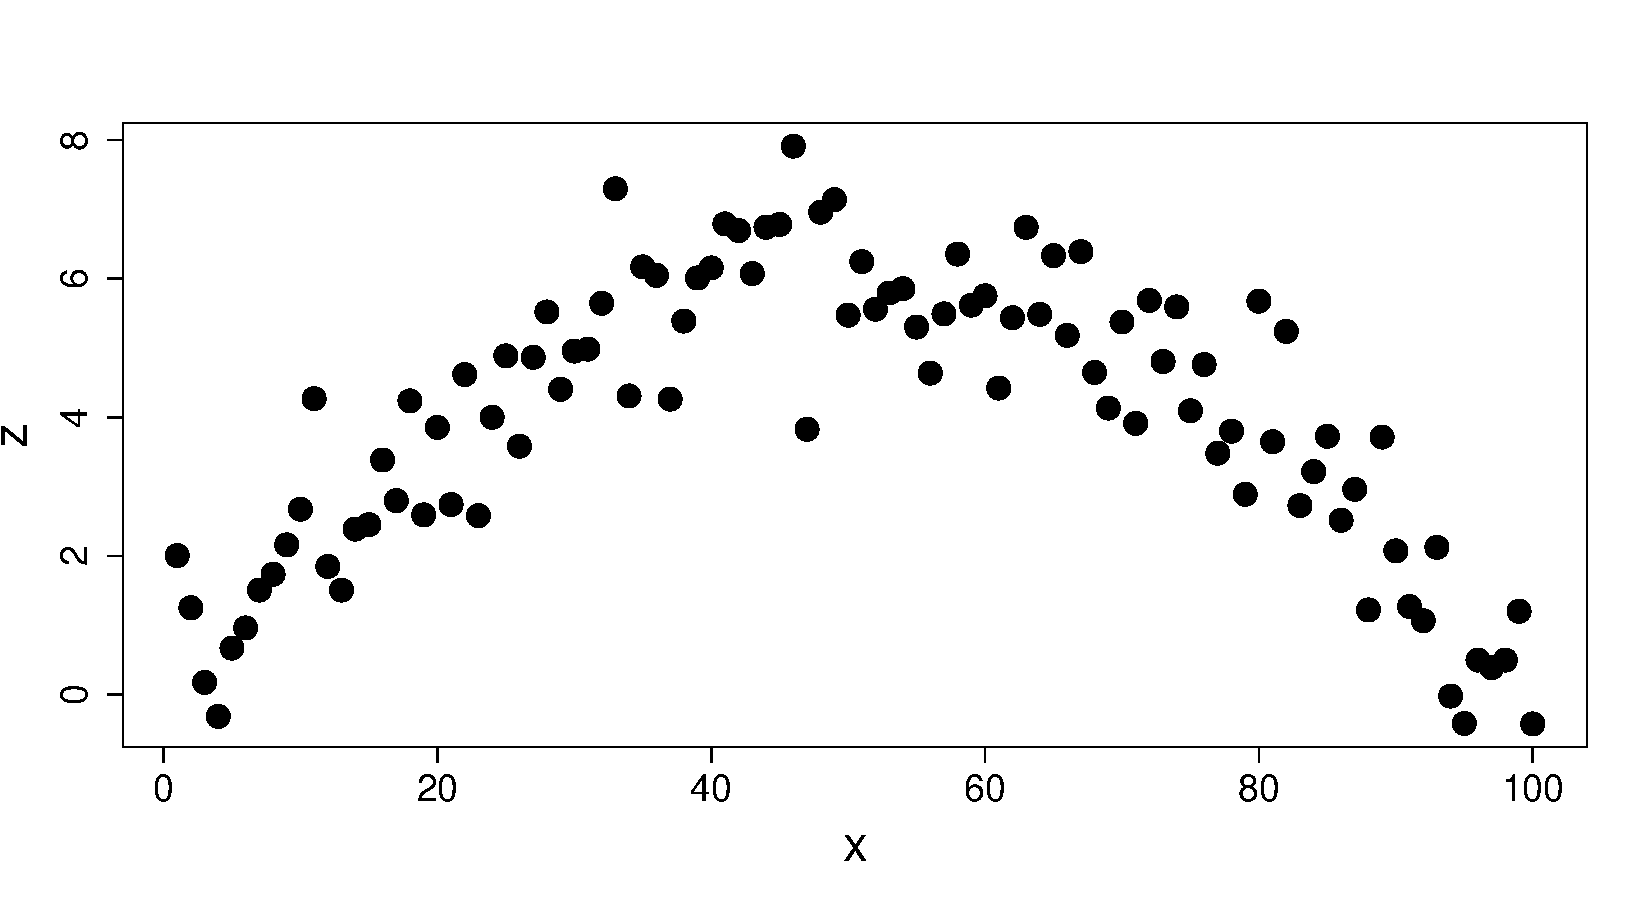
\includegraphics[width=.7\linewidth]{figure/AutoCor-DataFig} 

}



\end{knitrout}

\end{frame}

%-------------------------------------------------------------------------------
%                         Autocorrelation
%-------------------------------------------------------------------------------
\begin{frame} [fragile]
\frametitle{The Many Faces of ``Autocorrelation'': MODEL}
     
\begin{knitrout}\tiny
\definecolor{shadecolor}{rgb}{0.969, 0.969, 0.969}\color{fgcolor}\begin{kframe}
\begin{alltt}
x <- 1:100
gamma <- \hlfunctioncall{exp}(-x/50)
\hlfunctioncall{plot}(x, gamma, type = \hlstring{"l"}, lwd = 2, cex.lab = 2, cex.axis = 1.5, col = \hlstring{"blue"})
\end{alltt}
\end{kframe}

{\centering 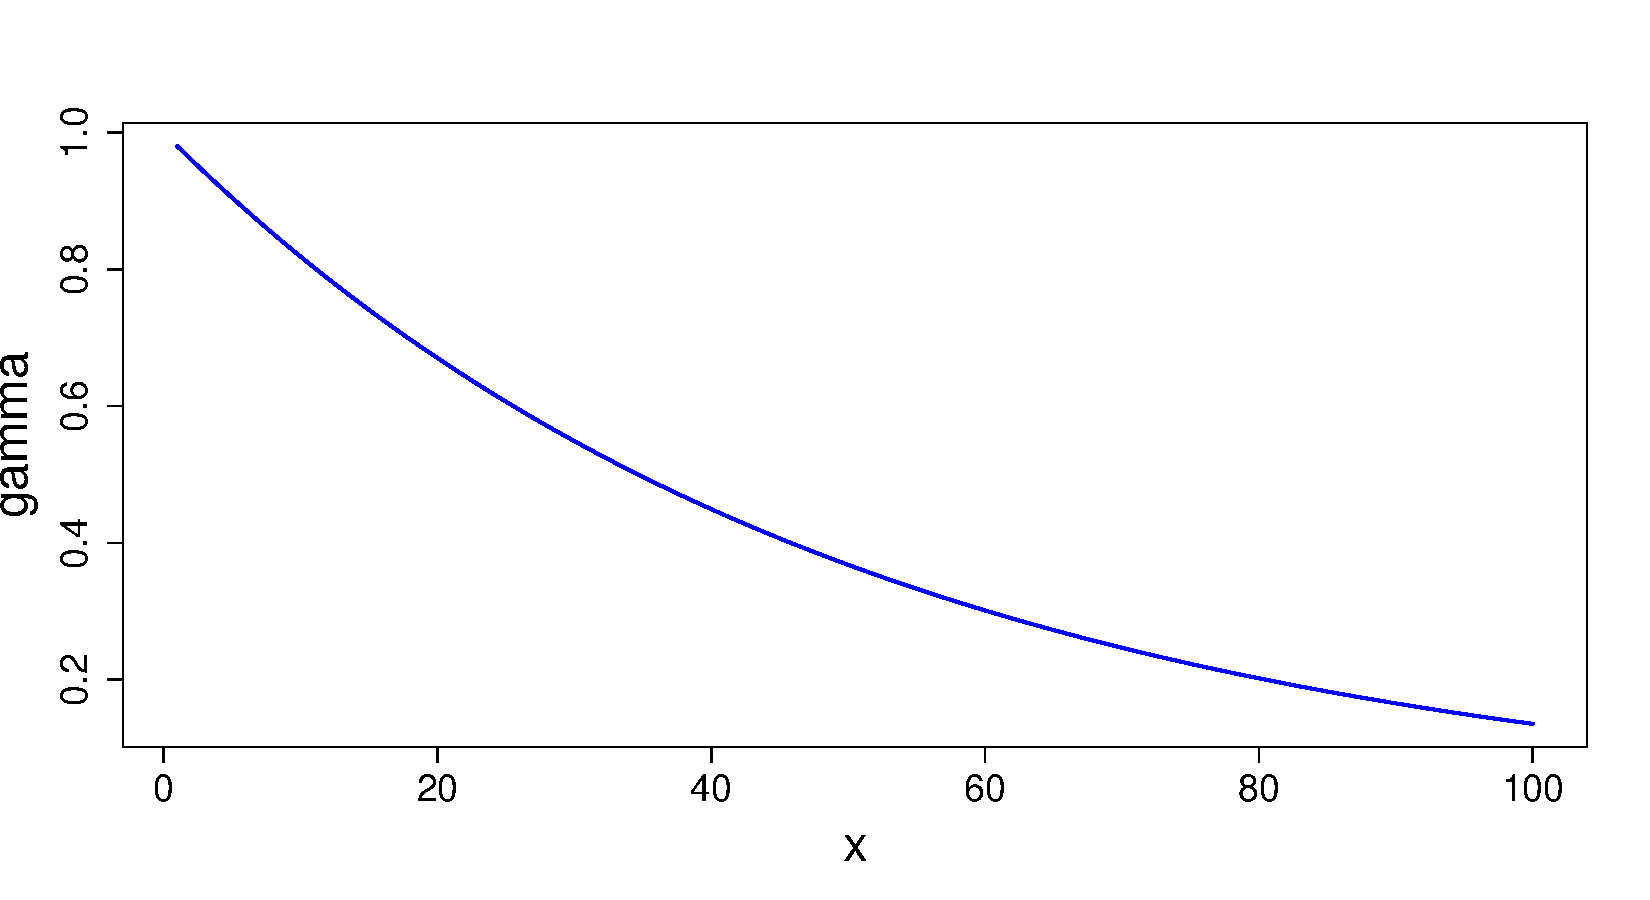
\includegraphics[width=.7\linewidth]{figure/AutoCor-ModelFig} 

}



\end{knitrout}

\end{frame}

%-------------------------------------------------------------------------------
%                         Autocorrelation
%-------------------------------------------------------------------------------
\begin{frame} [fragile]
\frametitle{The Many Faces of ``Autocorrelation'': PROCESS}
     
\begin{knitrout}\tiny
\definecolor{shadecolor}{rgb}{0.969, 0.969, 0.969}\color{fgcolor}\begin{kframe}
\begin{alltt}
\hlfunctioncall{set.seed}(4)
x <- 1:100
y <- \hlfunctioncall{rep}(1, times = 100)
xyz <- \hlfunctioncall{geoStatSim}(x, y, range = 100, nugget = 0.01, parsil = 6)
\hlfunctioncall{plot}(xyz$x, xyz$z, pch = 19, cex = 2, cex.lab = 2, cex.axis = 1.5)
\end{alltt}
\end{kframe}

{\centering 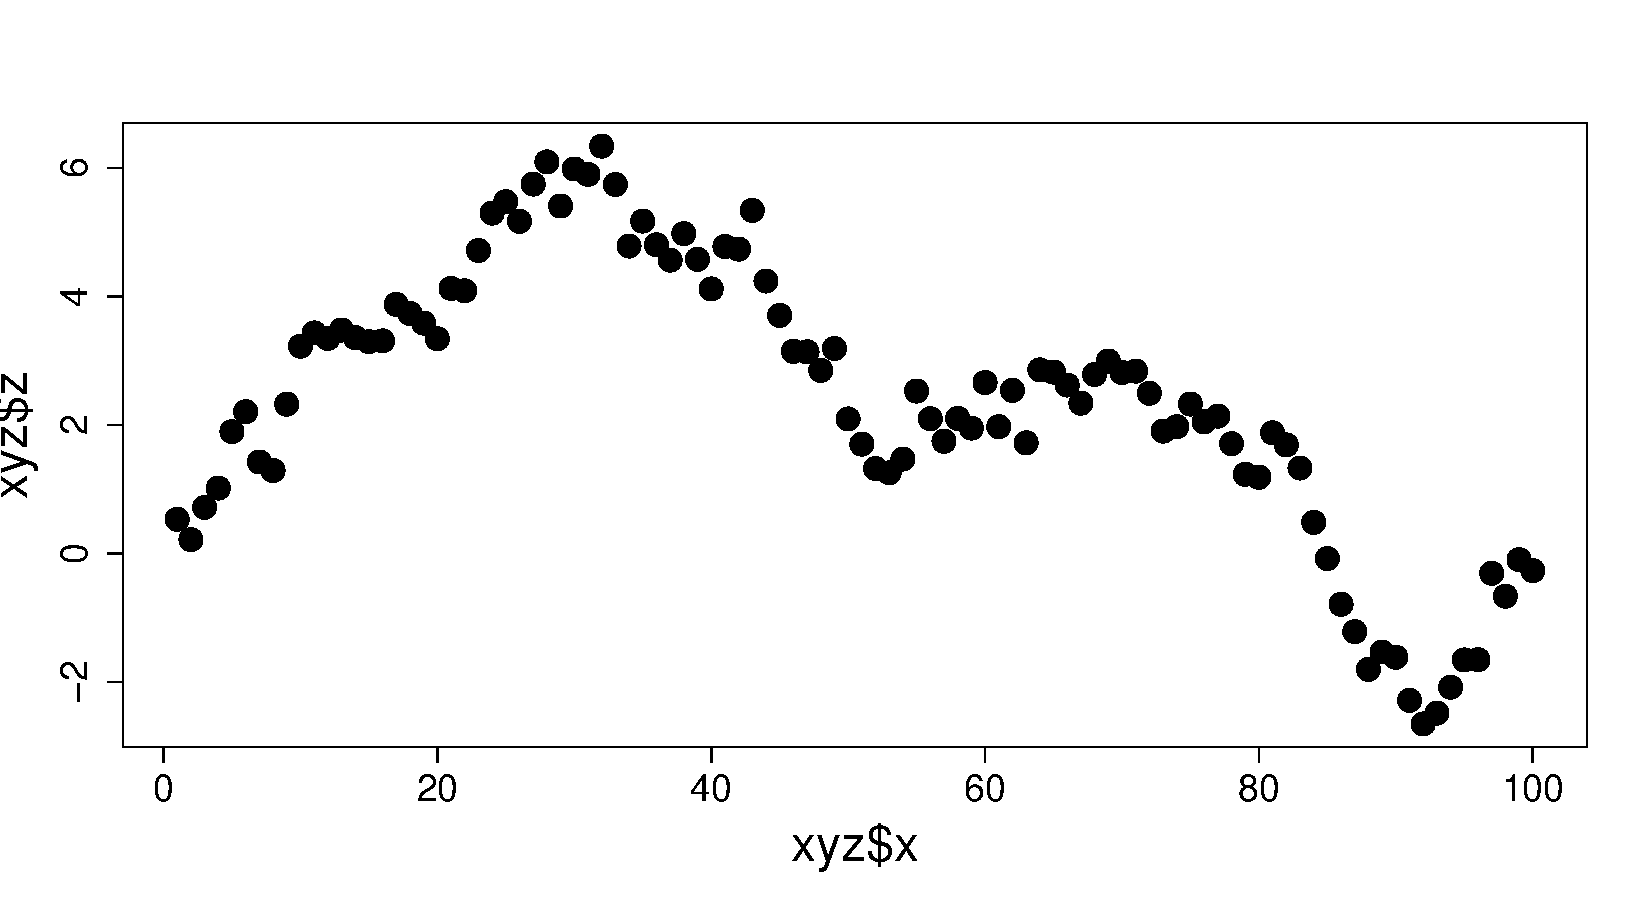
\includegraphics[width=.7\linewidth]{figure/AutoCor-ProcessFig} 

}



\end{knitrout}

\end{frame}

%-------------------------------------------------------------------------------
%                         Autocorrelation
%-------------------------------------------------------------------------------
\begin{frame} [fragile]
\frametitle{The Many Faces of ``Autocorrelation'': STATISTIC}
     
\begin{knitrout}\tiny
\definecolor{shadecolor}{rgb}{0.969, 0.969, 0.969}\color{fgcolor}\begin{kframe}
\begin{alltt}
spDF <- \hlfunctioncall{SpatialPointsDataFrame}(\hlfunctioncall{cbind}(xyz$x, xyz$y), \hlfunctioncall{data.frame}(z = xyz$z))
esv <- \hlfunctioncall{empSemivariogram}(spDF, \hlstring{"z"}, EmpVarMeth = \hlstring{"CovMean"})
\hlfunctioncall{plot}(esv$hx, esv$gamma, pch = 19, cex = esv$np/100, cex.lab = 2, cex.axis = 1.5)
\end{alltt}
\end{kframe}

{\centering 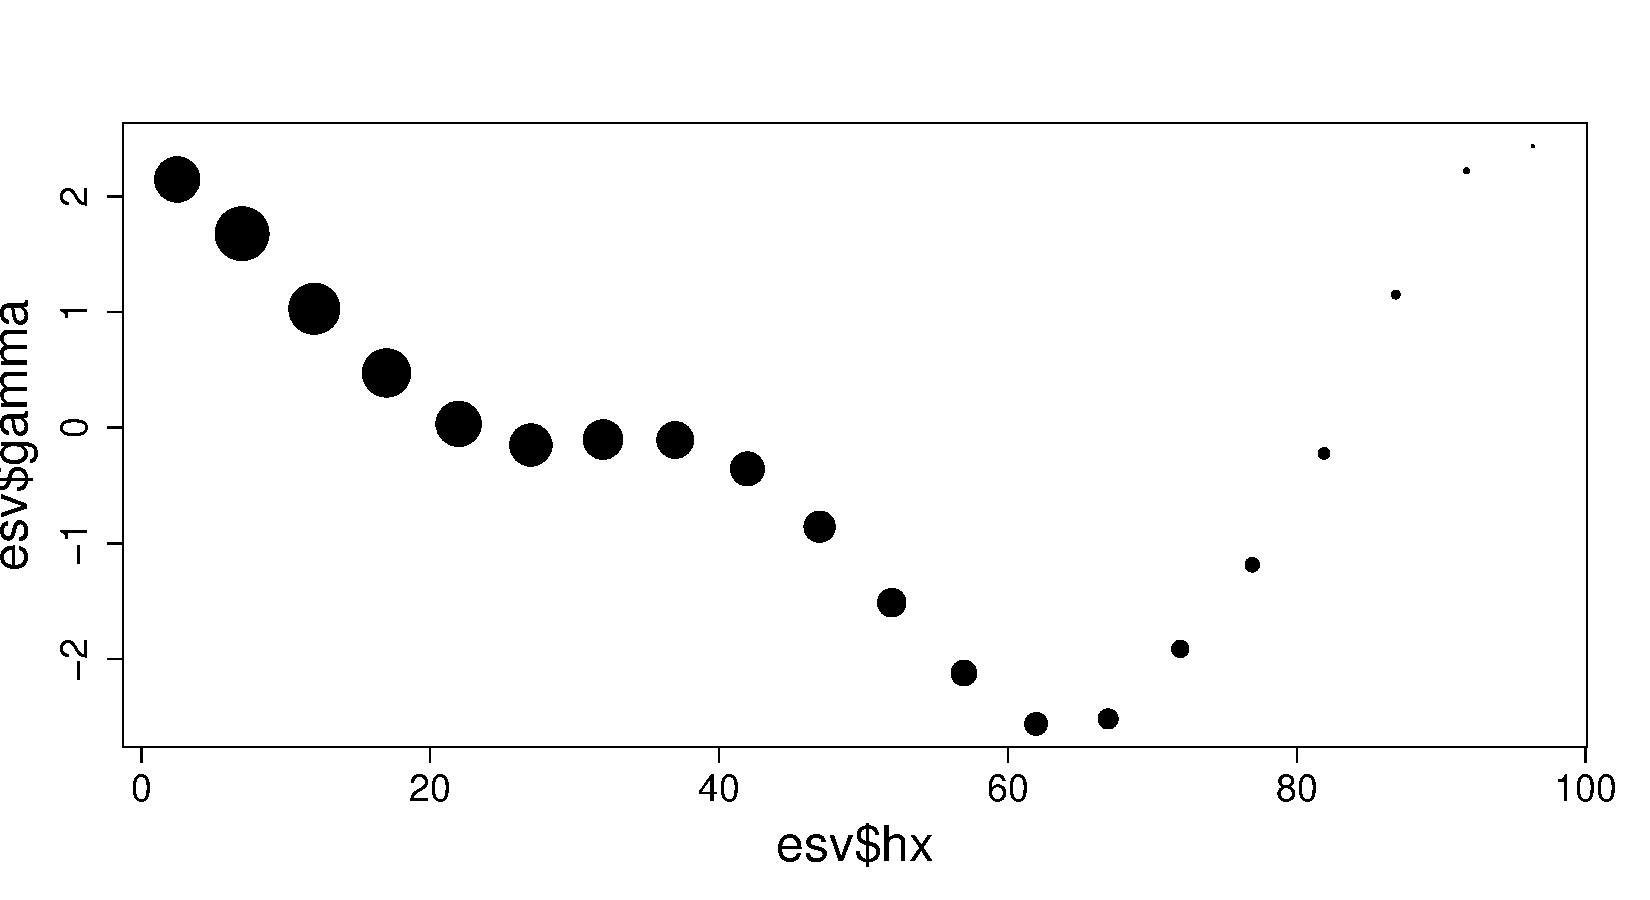
\includegraphics[width=.7\linewidth]{figure/AutoCor-StatisticFig} 

}



\end{knitrout}

\end{frame}

%-------------------------------------------------------------------------------
%                    Estimation Versus Prediction
%-------------------------------------------------------------------------------
\begin{frame} [fragile]
\frametitle{Estimation Versus Prediction}
	$E(\bz,Z_0) = \bone\mu, \quad \cov(\bz,Z_0) = \left(
		\begin{array}{cc}
			\bSigma & \bc \\
			\bc\upp & \sigma_0^2
		\end{array} \right)$ \\
  data mean = $\bone\upp\bz/n$ \\
	variance as estimator of $\mu$ = $\bone\upp\bSigma\bone/n^2$  \\
	variance as predictor = $E(\bone\upp\bz/n - Z_0)^2 = \bone\upp\bSigma\bone/n^2 -2\bone\upp\bc/n + \sigma_0^2$
\begin{knitrout}\tiny
\definecolor{shadecolor}{rgb}{0.969, 0.969, 0.969}\color{fgcolor}\begin{kframe}
\begin{alltt}
\hlcomment{# Independence}
SigmaInd <- \hlfunctioncall{diag}(6)
\hlcomment{# variance of mean estimator for first 5}
\hlfunctioncall{sum}(SigmaInd[1:5, 1:5])/5^2
\end{alltt}
\begin{verbatim}
## [1] 0.2
\end{verbatim}
\begin{alltt}
\hlcomment{# variance of first 5 to predict the 6th}
\hlfunctioncall{sum}(SigmaInd[1:5, 1:5])/5^2 - 2 * \hlfunctioncall{sum}(SigmaInd[6, 1:5])/5 + SigmaInd[6, 6]
\end{alltt}
\begin{verbatim}
## [1] 1.2
\end{verbatim}
\end{kframe}
\end{knitrout}

\end{frame}

%-------------------------------------------------------------------------------
%                    Estimation Versus Prediction
%-------------------------------------------------------------------------------
\begin{frame} [fragile]
\frametitle{Estimation Versus Prediction}
	$E(\bz,Z_0) = \bone\mu, \quad \cov(\bz,Z_0) = \left(
		\begin{array}{cc}
			\bSigma & \bc \\
			\bc\upp & \sigma_0^2
		\end{array} \right)$ \\
  data mean = $\bone\upp\bz/n$ \\
	variance as estimator of $\mu$ = $\bone\upp\bSigma\bone/n^2$  \\
	variance as predictor = $E(\bone\upp\bz/n - Z_0)^2 = \bone\upp\bSigma\bone/n^2 -2\bone\upp\bc/n + \sigma_0^2$
\begin{knitrout}\tiny
\definecolor{shadecolor}{rgb}{0.969, 0.969, 0.969}\color{fgcolor}\begin{kframe}
\begin{alltt}
\hlcomment{# lots of autocorrelation}
SigmaAC <- \hlfunctioncall{matrix}(0.9999, nrow = 6, ncol = 6)
\hlfunctioncall{diag}(SigmaAC) <- 1
\hlcomment{# variance of mean estimator for first 5}
\hlfunctioncall{sum}(SigmaAC[1:5, 1:5])/5^2
\end{alltt}
\begin{verbatim}
## [1] 0.9999
\end{verbatim}
\begin{alltt}
\hlcomment{# variance of first 5 to predict the 6th}
\hlfunctioncall{sum}(SigmaAC[1:5, 1:5])/5^2 - 2 * \hlfunctioncall{sum}(SigmaAC[6, 1:5])/5 + SigmaAC[6, 6]
\end{alltt}
\begin{verbatim}
## [1] 0.00012
\end{verbatim}
\end{kframe}
\end{knitrout}

\end{frame}

%-------------------------------------------------------------------------------
%                    Estimation Versus Prediction
%-------------------------------------------------------------------------------
\begin{frame} [fragile]
\frametitle{Estimation Versus Prediction}
\tiny
	\vspace{.2cm}
	\begin{tabular} {p{4.5cm} p{4.5cm}}
		$\left(\begin{array}{rrrrrr}
				1.0000 & 0.9999 & 0.9999 & 0.9999 & 0.9999 & 0.9999 \\ 
				0.9999 & 1.0000 & 0.9999 & 0.9999 & 0.9999 & 0.9999 \\ 
				0.9999 & 0.9999 & 1.0000 & 0.9999 & 0.9999 & 0.9999 \\ 
				0.9999 & 0.9999 & 0.9999 & 1.0000 & 0.9999 & 0.9999 \\ 
				0.9999 & 0.9999 & 0.9999 & 0.9999 & 1.0000 & 0.9999 \\ 
				0.9999 & 0.9999 & 0.9999 & 0.9999 & 0.9999 & 1.0000  
		\end{array}\right)$ &
		\hspace{1.5cm} $\left(\begin{array}{rrrrrr}
				1 & 0 & 0 & 0 & 0 & 0 \\ 
				0 & 1 & 0 & 0 & 0 & 0 \\ 
				0 & 0 & 1 & 0 & 0 & 0 \\ 
				0 & 0 & 0 & 1 & 0 & 0 \\ 
				0 & 0 & 0 & 0 & 1 & 0 \\ 
				0 & 0 & 0 & 0 & 0 & 1 
 		\end{array}\right)$ 
	\end{tabular}
\begin{knitrout}\tiny
\definecolor{shadecolor}{rgb}{0.969, 0.969, 0.969}\color{fgcolor}\begin{kframe}
\begin{alltt}
\hlfunctioncall{set.seed}(18)
z.AC <- \hlfunctioncall{t}(\hlfunctioncall{chol}(SigmaAC)) %*% \hlfunctioncall{rnorm}(6)
z.ind <- \hlfunctioncall{t}(\hlfunctioncall{chol}(SigmaInd)) %*% \hlfunctioncall{rnorm}(6)
\hlfunctioncall{plot}(1:5, z.AC[1:5], ylim = \hlfunctioncall{c}(-3, 3), xlim = \hlfunctioncall{c}(1, 6), pch = 19, cex = 2, col = \hlstring{"green"})
\hlfunctioncall{points}(6, z.AC[6], pch = 19, cex = 2, col = \hlstring{"red"})
\hlfunctioncall{lines}(\hlfunctioncall{c}(0, 6), \hlfunctioncall{c}(0, 0), lwd = 3)
\hlfunctioncall{plot}(1:5, z.ind[1:5], ylim = \hlfunctioncall{c}(-3, 3), xlim = \hlfunctioncall{c}(1, 6), pch = 19, cex = 2, col = \hlstring{"green"})
\hlfunctioncall{points}(6, z.ind[6], pch = 19, cex = 2, col = \hlstring{"red"})
\hlfunctioncall{lines}(\hlfunctioncall{c}(0, 6), \hlfunctioncall{c}(0, 0), lwd = 3, pch = 19, cex = 2)
\end{alltt}
\end{kframe}
\end{knitrout}



	\begin{tabular} {p{4.5cm} p{4.5cm}}
		\begin{center}
		  \vspace{-1.3cm}
			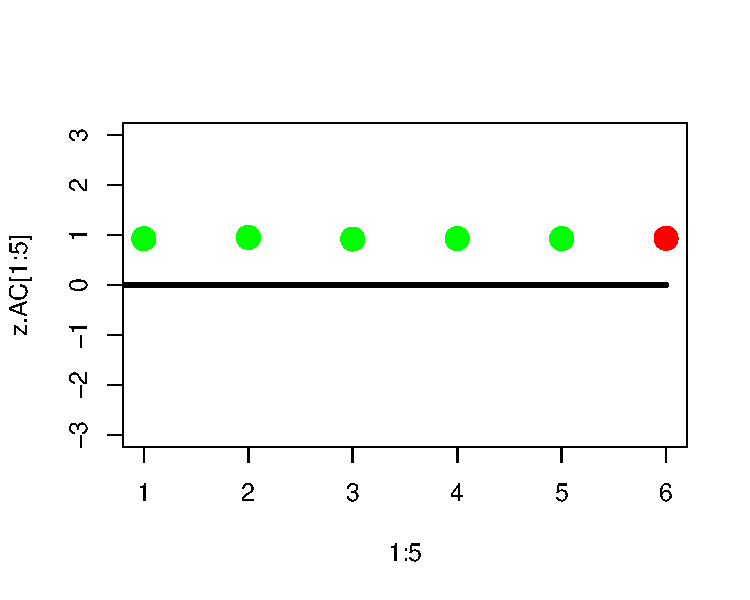
\includegraphics[width=4.0cm]{figure/AutoCor-EstPredFig1} 
		\end{center} &
		\begin{center}
		  \vspace{-1.3cm}
			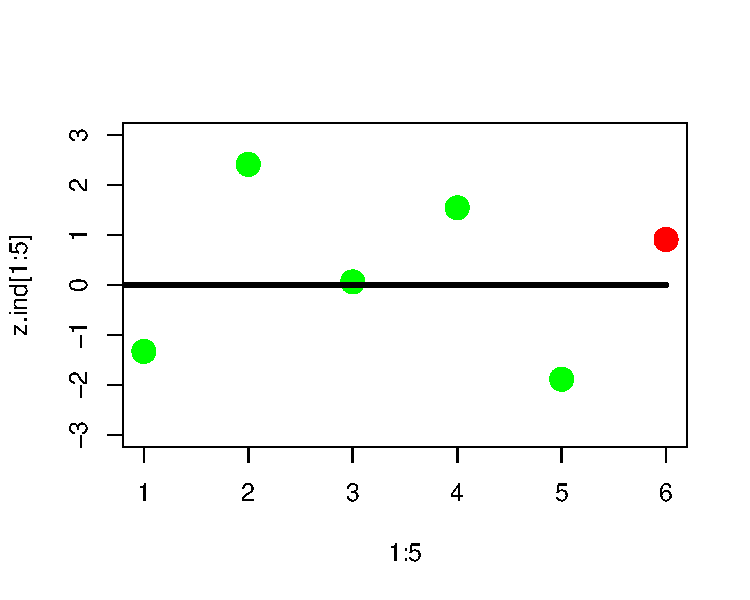
\includegraphics[width=4.0cm]{figure/AutoCor-EstPredFig2} 
		\end{center} 
	\end{tabular}
\end{frame}

%-------------------------------------------------------------------------------
%                    Notatation
%-------------------------------------------------------------------------------
\section{Types of Spatial Data}
\subsection{}
\begin{frame} [fragile]
\frametitle{Notation}




	\vspace{.2cm}
	\begin{tabular} {p{4cm} p{5cm}}

 		\vspace{.2cm}
		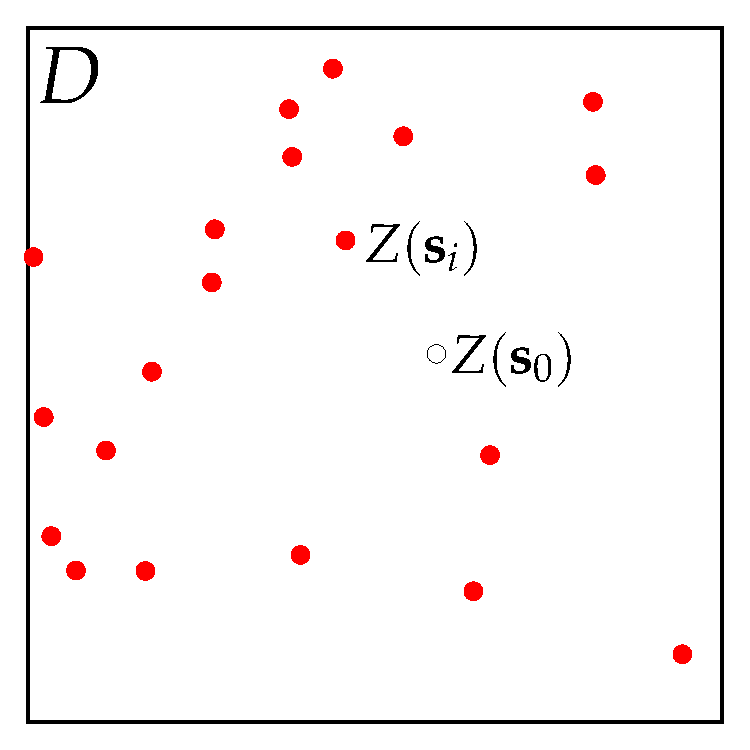
\includegraphics[width=4.0cm]{figure/Notation-plot} &
		\vspace{.5cm}
		\bit
			\item{$D$ is the spatial region or area of interest} 
			\item{$\bs$ contains the spatial coordinates}
			\item{$Z$ is the value located at the spatial coordinates}
		\eit

	\end{tabular}

\end{frame}

%-------------------------------------------------------------------------------
%                    Types of Spatial Data
%-------------------------------------------------------------------------------
\begin{frame} [fragile]
\frametitle{Types of Spatial Data}

	\vspace{.2cm}
	\begin{tabular} {p{4cm} p{5cm}}

 		\vspace{.2cm}
		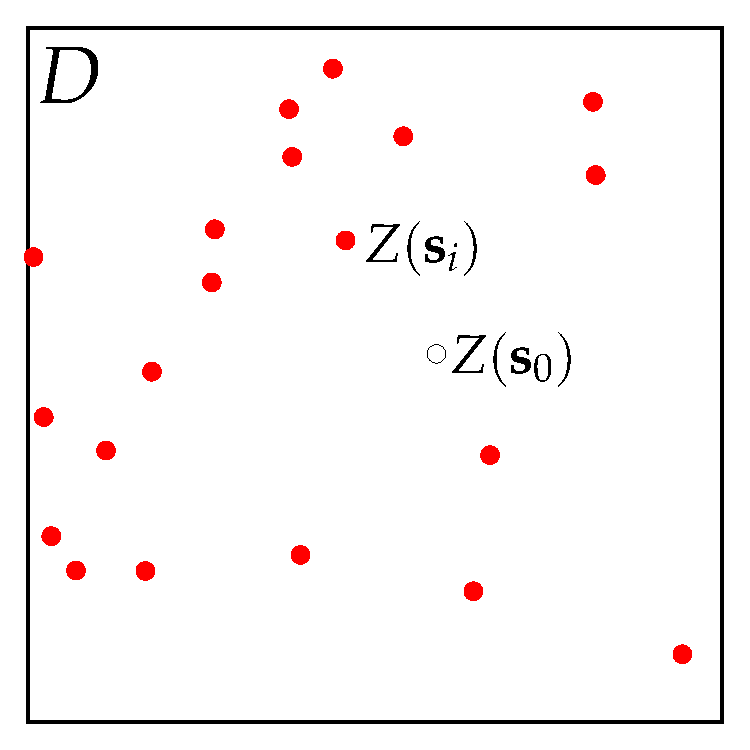
\includegraphics[width=4.0cm]{figure/Notation-plot} &
		\vspace{-.2cm}
		\bit
			\item{$\{Z(\bs):\bs \in D\}$}
			\item{{\color{blue!70!black}Geostatistical Data:} $Z$ random, $D$ fixed, continuous, infinite} 
			\item{{\color{blue!70!black}Lattice/Aerial Data:} $Z$ random, $D$ fixed, finite, (ir)regular grid} 
			\item{{\color{blue!70!black}Point Pattern Data:} $Z \equiv 1$, $D$ random, finite} 
		\eit

	\end{tabular}

\end{frame}

%-------------------------------------------------------------------------------
%                    Types of Spatial Data
%-------------------------------------------------------------------------------
\begin{frame} [fragile]
\frametitle{Examples of Geostatistical Data}


	\begin{tabular} {p{4.5cm} p{4.5cm}}

\begin{knitrout}\tiny
\definecolor{shadecolor}{rgb}{0.969, 0.969, 0.969}\color{fgcolor}

{\centering 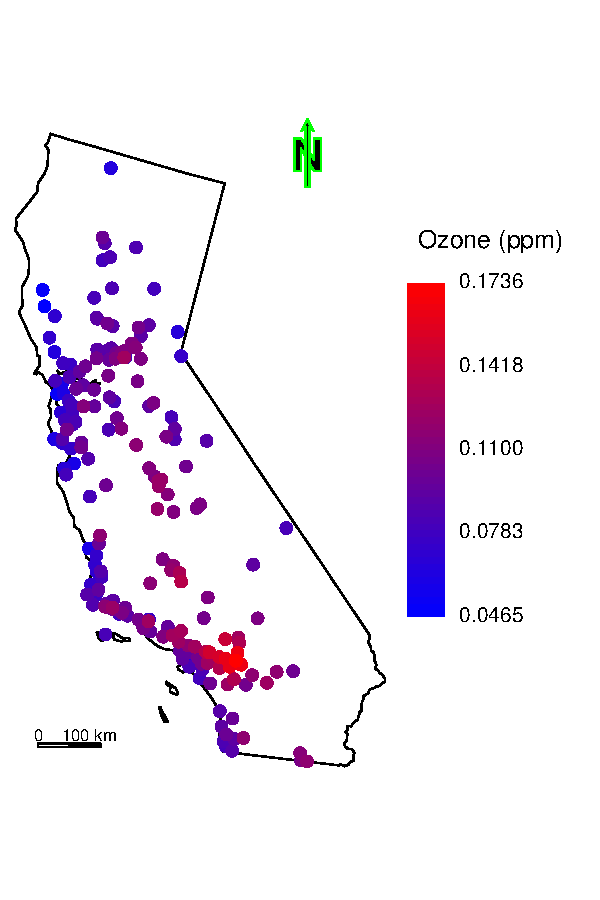
\includegraphics[width=\maxwidth]{figure/colorPointsCAOzone-plot} 

}



\end{knitrout}

 &


\begin{knitrout}\tiny
\definecolor{shadecolor}{rgb}{0.969, 0.969, 0.969}\color{fgcolor}

{\centering 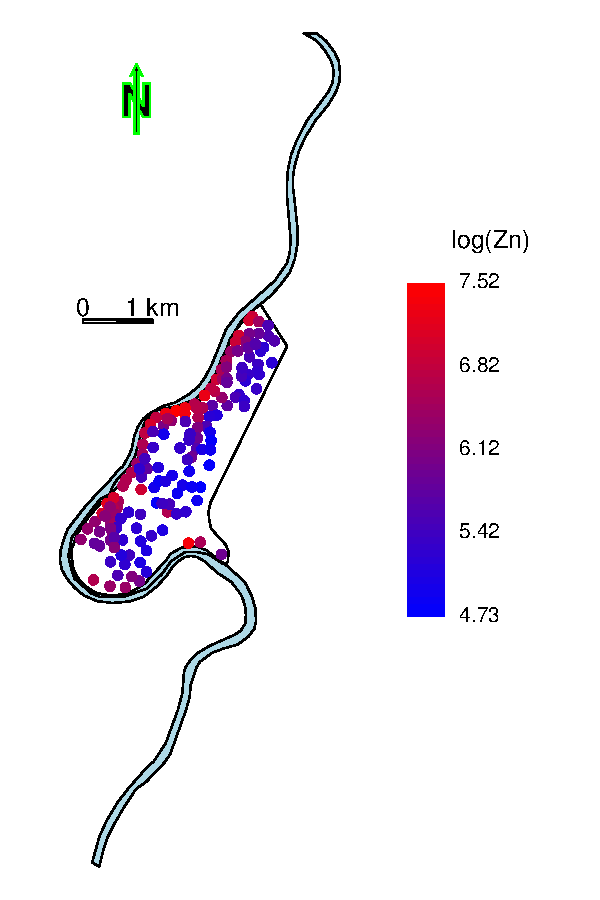
\includegraphics[width=\maxwidth]{figure/colorPointsMeuseLogZN-plot} 

}



\end{knitrout}

	\end{tabular}

\end{frame}

%-------------------------------------------------------------------------------
%                    Types of Spatial Data
%-------------------------------------------------------------------------------
\begin{frame}[fragile]
\frametitle{Examples of Lattice/Aerial Data}







	\begin{tabular} {c}


	{\centering 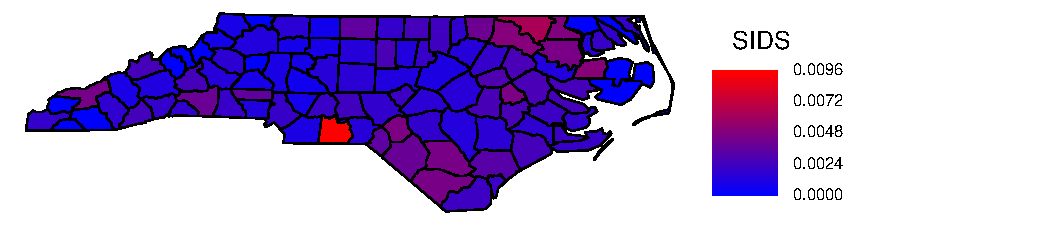
\includegraphics[width=\maxwidth]{figure/rawSIDS-plot} }
 	\\



	{\centering 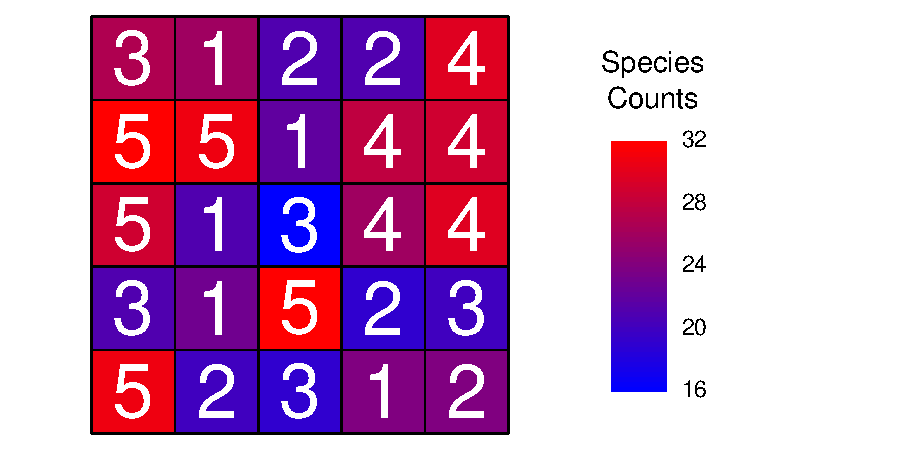
\includegraphics[width=.6\maxwidth]{figure/fireDiv-plot} }


	\end{tabular}

\end{frame}

%-------------------------------------------------------------------------------
%                    Types of Spatial Data
%-------------------------------------------------------------------------------
\begin{frame}[fragile]
\frametitle{Examples of Point Pattern Data}











	\begin{tabular} {p{4.5cm} p{4.5cm}}
	{\centering 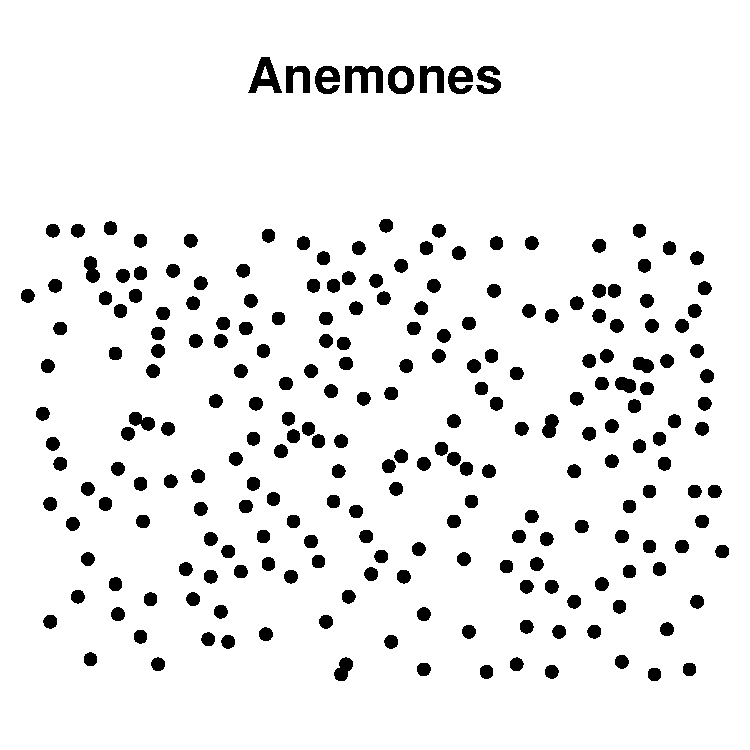
\includegraphics[width=\maxwidth]{figure/anemones-plot} } &
	{\centering 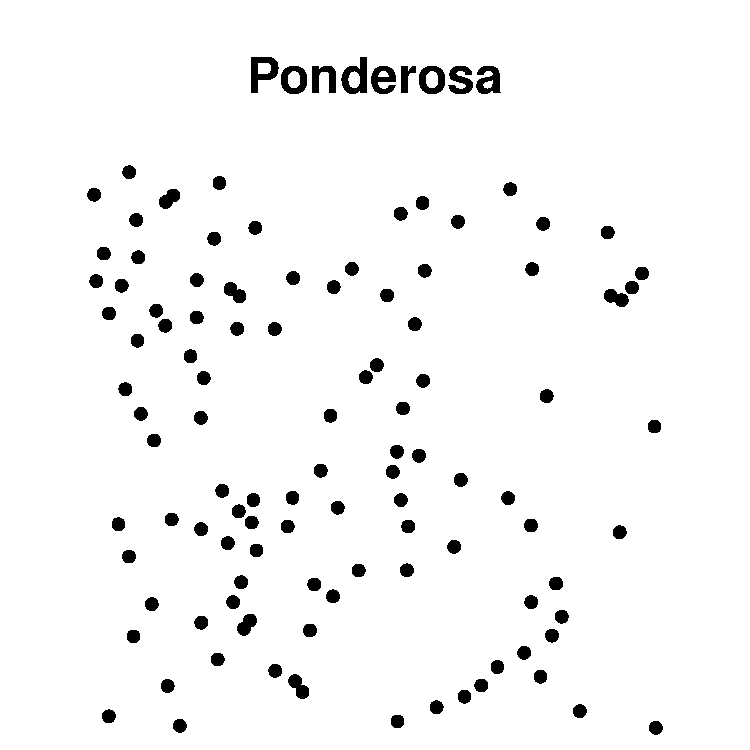
\includegraphics[width=\maxwidth]{figure/ponderosa-plot} }

	\end{tabular}

\end{frame}

%-------------------------------------------------------------------------------
%                    Estimation
%-------------------------------------------------------------------------------

\section{Estimation}
\subsection{}
\begin{frame}[fragile]
\frametitle{Estimation}

minimize for $\btheta$ \\
\begin{center}
	$-2\ell(\btheta,\bz) \propto \log|\bSigma_{\btheta}| + \br_{\btheta}\upp\bSigma\upi\br_{\btheta}$
\end{center}
or
\begin{center}
	$-2\ell_{\textrm{REML}}(\btheta,\bz) \propto \log|\bSigma_{\btheta}| + \br_{\btheta}\upp\bSigma_{\btheta}\upi\br_{\btheta} + \log|\bX\upp\bSigma_{\btheta}\upi\bX|$
\end{center}
where
\begin{center}
	$\br_{\btheta} = \bz - \bX\hat{\bbeta}_{\btheta}$
\end{center}
and
\begin{center}
	$\hat{\bbeta}_{\btheta} = (\bX\upp\bSigma_{\btheta}\upi\bX)\upi\bX\upp\bSigma\upi\bz$
\end{center}

\end{frame}

%-------------------------------------------------------------------------------
%                    Prediction
%-------------------------------------------------------------------------------
\section{Prediction}
\subsection{}
\begin{frame}[fragile]
\frametitle{Prediction}

		 \[
			\left(\begin{array}{c}	
					\bz_{\textrm{observed}} \\
					{\color{green!70!black} \bz_{\textrm{unobserved}}}
			\end{array} \right) =  \bX{\color{yellow!70!black}\bbeta} + 
			\bepsilon, \ \var(\bepsilon) = \bSigma({\color{red!70!black}\btheta}) \] \\





	\begin{tabular} {p{4.5cm} p{4.5cm}}
		\vspace{-.8cm}
		{\centering 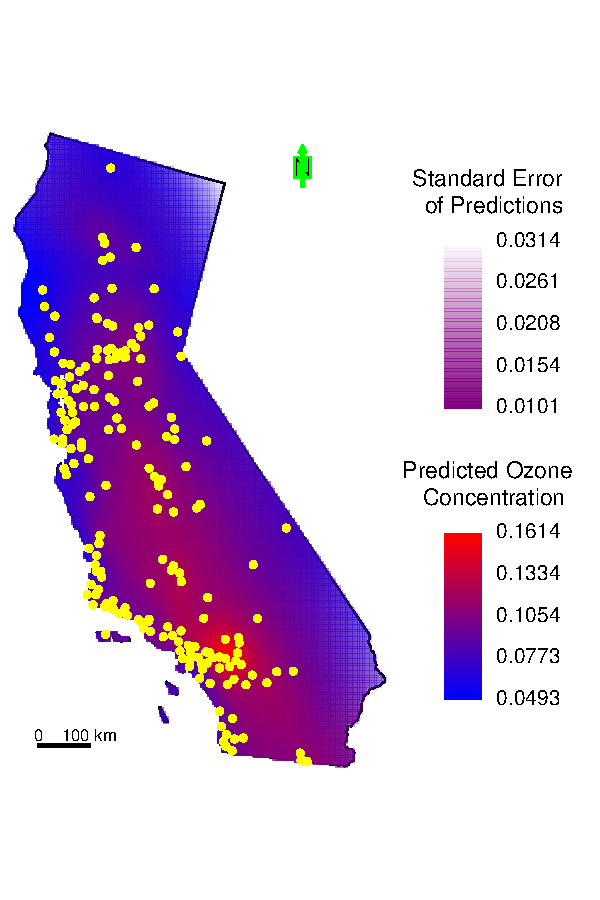
\includegraphics[width=.9\maxwidth]{figure/CA-predMap} } &
		\vspace{-.8cm}
		{\centering 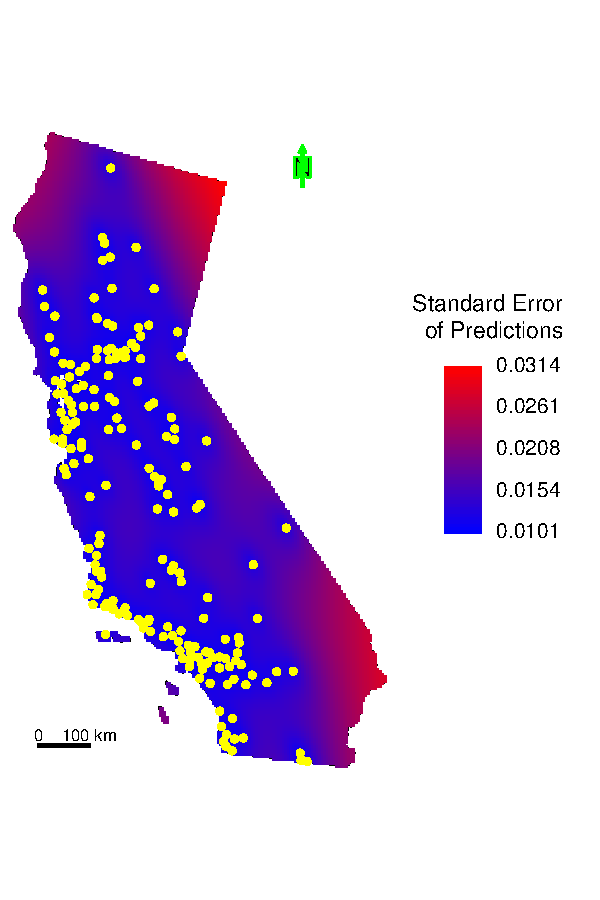
\includegraphics[width=.9\maxwidth]{figure/CA-predSEMap} }

	\end{tabular}

\end{frame}

%-------------------------------------------------------------------------------
%                    Regression
%-------------------------------------------------------------------------------
\section{Regression}
\subsection{}
\begin{frame}[fragile]
\frametitle{Spatial Regression}








	\begin{tabular} {p{4.5cm} p{4.5cm}}
		\vspace{.1cm}
		\begin{tabular} {c}
				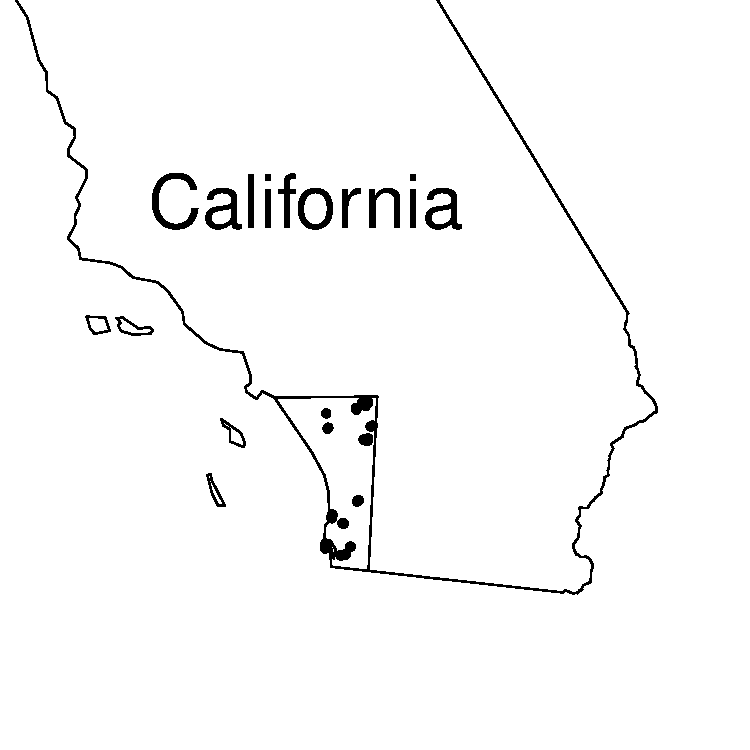
\includegraphics[width=3.8cm]{figure/lizardCA-plot} \\
				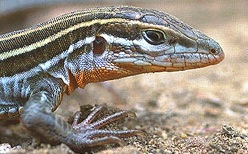
\includegraphics[width=3.8cm]{figure/whiptailHead.jpg}
		\end{tabular} &

		\begin{itemize}
			\item Whiptail Lizard
			\item 148 locations in Southern California
			\item Measured the average number caught in traps over 80-90 trapping events in one year
			\item Data log-transformed, one outlier removed
		\end{itemize}

	\end{tabular}

\end{frame}

%-------------------------------------------------------------------------------
%                    Regression
%-------------------------------------------------------------------------------
\begin{frame}[fragile]
\frametitle{Whiptail Lizard Data}








		 \[
			\left(\begin{array}{c}	
					\bz_{\textrm{observed}} \\
					{\color{green!70!black} \bz_{\textrm{unobserved}}}
			\end{array} \right) =  \bX{\color{yellow!70!black}\bbeta} + 
			\bepsilon, \ \var(\bepsilon) = \bSigma({\color{red!70!black}\btheta}) \] \\

	\vspace{-.4cm} \begin{tabular}{p{4.5cm} p{4.5cm}}
		\bit
			\item {\color{yellow!70!black}Ant Abundance}
			\item {\color{yellow!70!black}Percent Sandy Soil}
		\eit &
		\bit
			\item {\color{red!70!black}Matern Model}
			\item {\color{red!70!black}Anisotropy}
		\eit
	\end{tabular}

	\begin{tabular} {p{5cm} p{4cm}}
			\vspace{-.7cm}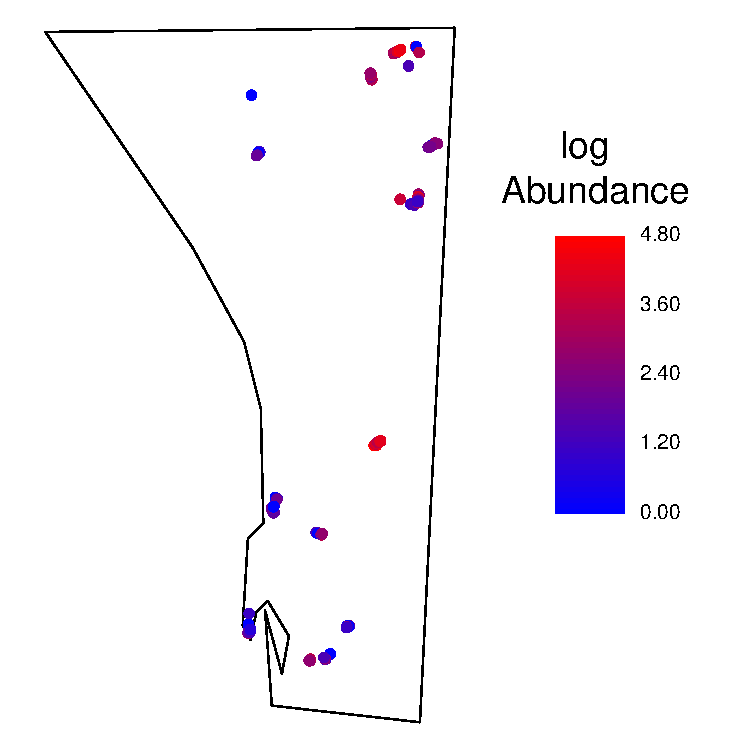
\includegraphics[width=4.0cm]{figure/lizardPoints-plot}  &
		\vspace{-.7cm} \begin{tabular} {c}
			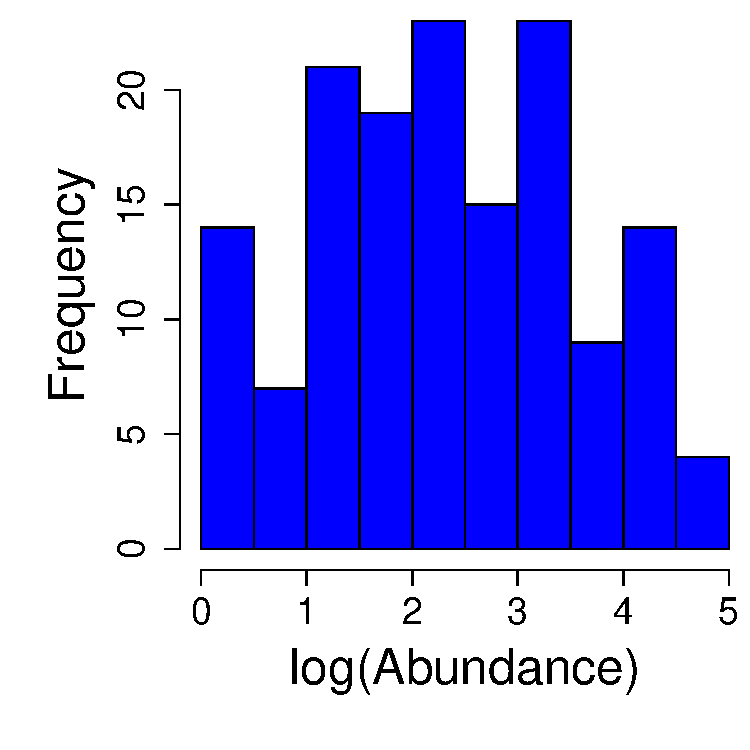
\includegraphics[width=1.9cm]{figure/lizardHist-plot} \\
			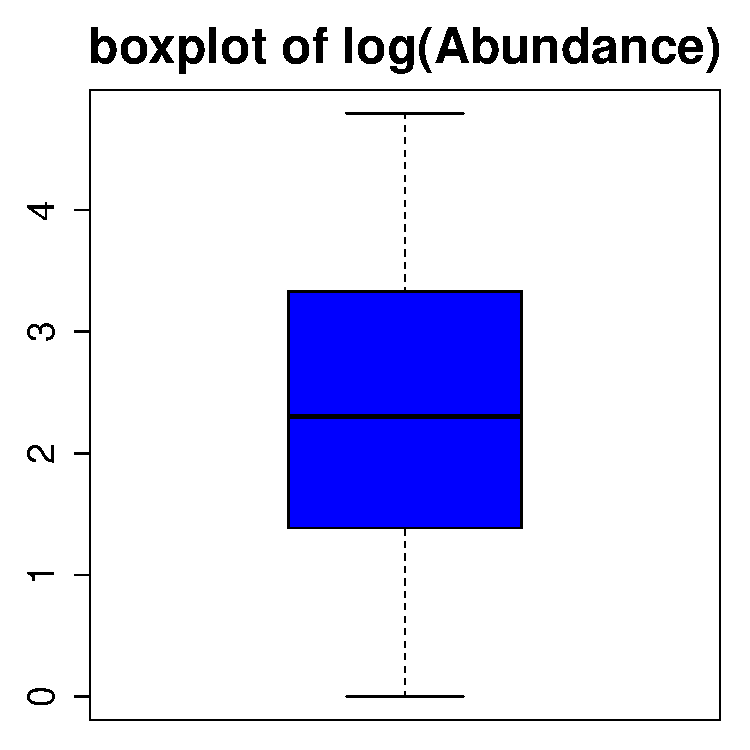
\includegraphics[width=1.9cm]{figure/lizardBox-plot}
		\end{tabular}
	\end{tabular}

\end{frame}

%-------------------------------------------------------------------------------
%                    Regression
%-------------------------------------------------------------------------------
\begin{frame}[fragile]
\frametitle{Fitted Model for Whiptail Lizard Data}



	
		 \[
			\left(\begin{array}{c}	
					\bz_{\textrm{observed}} \\
					{\color{green!70!black} \bz_{\textrm{unobserved}}}
			\end{array} \right) =  \bX{\color{yellow!70!black}\bbeta} + 
			\bepsilon, \ \var(\bepsilon) = \bSigma({\color{red!70!black}\btheta}) \] \\




	\begin{table}[ht]
	\centering
	\begin{tabular}{rrrrrr}
	 Effect & Est & Std Error & $t$-value & df & Pr($t$:H$_0$) \\ 
		\cye{Intercept} & \cye{0.716} & \cye{0.574} & \cye{146} & \cye{1.25} & \cye{0.2139} \\ 
		\cye{Ant Abund} & \cye{0.252} & \cye{0.107} & \cye{146} & \cye{2.36} & \cye{0.0195} \\ 
		\cye{Sandy Soil} & \cye{0.764} & \cye{0.249} & \cye{146} & \cye{3.07} & \cye{0.0026} \\ 
	\end{tabular}
	\end{table}




\scriptsize

	% latex table generated in R 3.0.1 by xtable 1.7-1 package
	% Thu May 23 09:29:45 2013
	\begin{table}[ht]
	\centering
	\begin{tabular}{rrr}
	Component & Parameter & Estimate \\ 
	\cre{nugget} & \cre{nugget} & \cre{0.598} \\ 
	\cre{besselK} & \cre{parsil} & \cre{1.027} \\ 
	\cre{besselK} & \cre{range} & \cre{160313} \\ 
	\cre{besselK} & \cre{minorp} & \cre{0.042} \\ 
	\cre{besselK} & \cre{rotate} & \cre{18.5} \\ 
	\cre{besselK} & \cre{extrap} & \cre{0.539} \\ 
	\end{tabular}
	\end{table}


\end{frame}
	
%-------------------------------------------------------------------------------
%                        Spatial Design of Experiments
%-------------------------------------------------------------------------------

\section{DOX}
\subsection{}
\begin{frame} 
\frametitle{Glades in the Ozarks}
     
		\begin{center}
		  \vspace{-.5cm}
			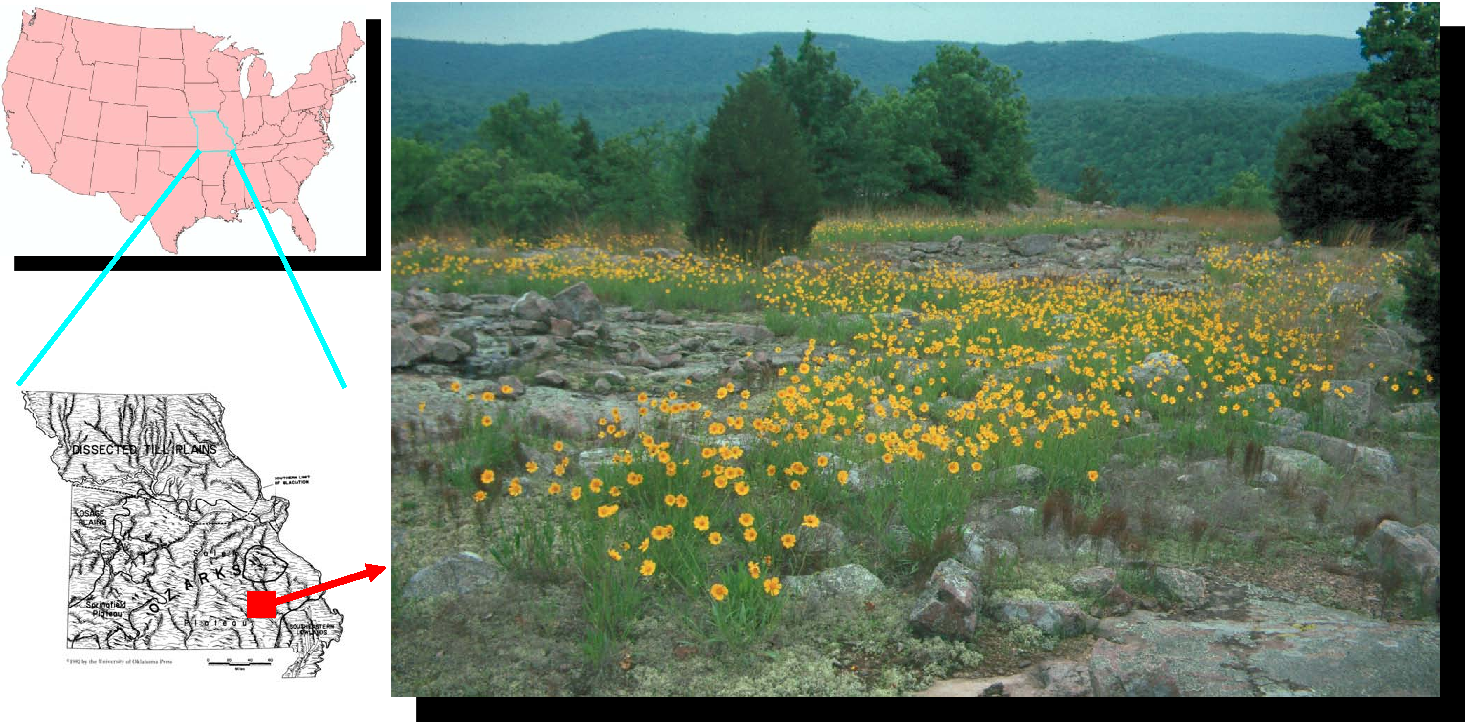
\includegraphics[width=10.4cm]{figure/OzarkDesign1Crop.pdf} 
		\end{center} 

\end{frame}

%-------------------------------------------------------------------------------
%                        Spatial Design of Experiments
%-------------------------------------------------------------------------------

\begin{frame} 
\frametitle{Simulated Spatial Experimental Design}
     
		\begin{center}
		  \vspace{-.5cm}
			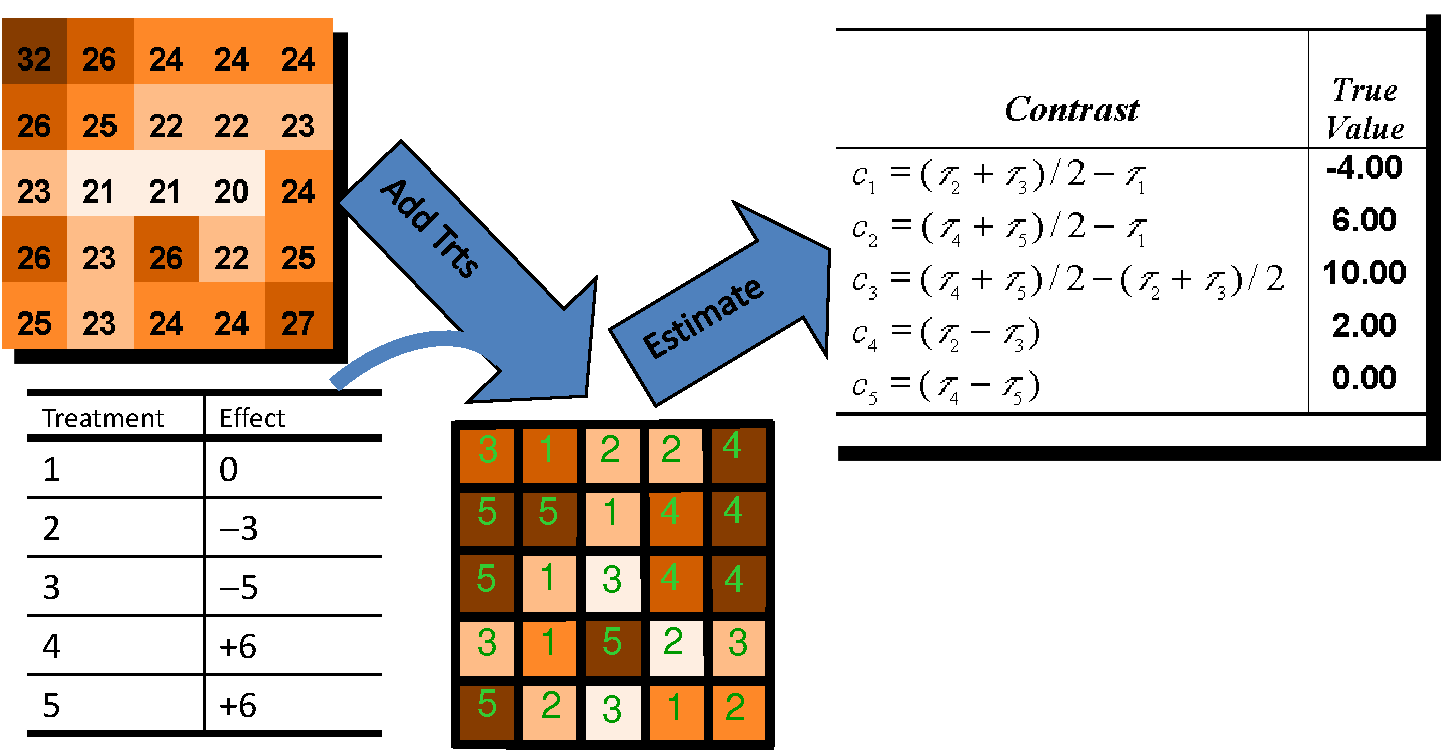
\includegraphics[width=10.4cm]{figure/OzarkDesign2Crop.pdf} 
		\end{center} 

\end{frame}

%-------------------------------------------------------------------------------
%                        Spatial Design of Experiments
%-------------------------------------------------------------------------------

\begin{frame} 
\frametitle{Simulated Spatial Experimental Design}



	




\scriptsize

		 \[
			\left(\begin{array}{c}	
					\bz_{\textrm{observed}} \\
					{\color{green!70!black} \bz_{\textrm{unobserved}}}
			\end{array} \right) =  \bX{\color{yellow!70!black}\bbeta} + 
			\bepsilon, \ \var(\bepsilon) = \bSigma({\color{red!70!black}\btheta}) \] \\

% latex table generated in R 3.0.1 by xtable 1.7-1 package
% Thu May 23 11:52:36 2013
\begin{table}[ht]
\centering
\begin{tabular}{rrrrrr}
True Value & Ind Est & Ind SE & Sp Est & Sp SE \\ 
  \hline
-4 & \cye{-2.4} & \cye{1.29} & \cye{-2.95} & \cye{0.87} \\ 
6 & \cye{6.6} & \cye{1.29} & \cye{6.81} & \cye{1.05} \\ 
10 & \cye{9.0} & \cye{1.05} & \cye{9.77} & \cye{0.84} \\ 
2 & \cye{0.4} & \cye{1.49} & \cye{0.53} & \cye{1.07} \\ 
0 & \cye{-2.4} & \cye{1.49} & \cye{-1.94} & \cye{1.68} \\ 
   \hline
& nugget: \cre{5.56} & & nugget: \cre{0.00} & \\
& & & partial sill: \cre{13.55} & \\
& & & range:  \cre{9.36} & \\
\end{tabular}
\end{table}

		\vspace{-.5cm}
		\begin{center}
			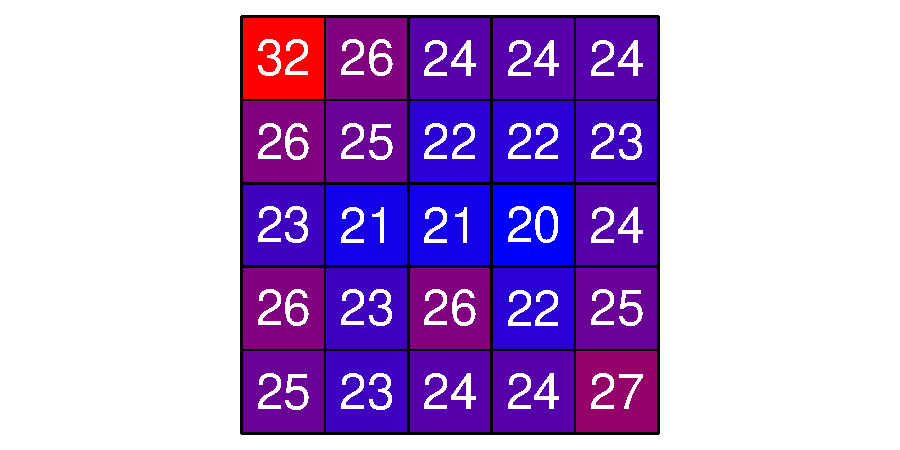
\includegraphics[width=4cm]{figure/fireDivOrig-plot} 
			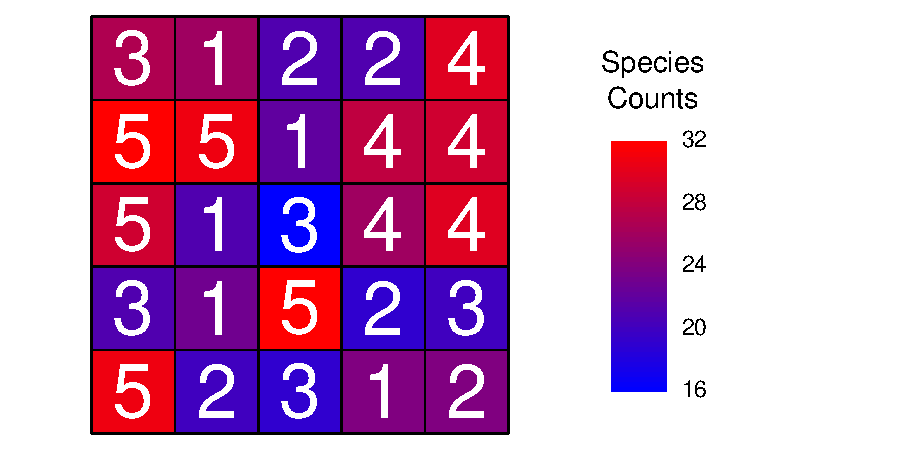
\includegraphics[width=4cm]{figure/fireDiv-plot} 
		\end{center} 

\end{frame}

%-------------------------------------------------------------------------------
%                        Spatial Sampling
%-------------------------------------------------------------------------------

\section{Sampling}
\subsection{Spatial Sampling}
\begin{frame} 
     
	\begin{tabular} {p{6cm} p{3cm}}
		\vspace{.1cm} 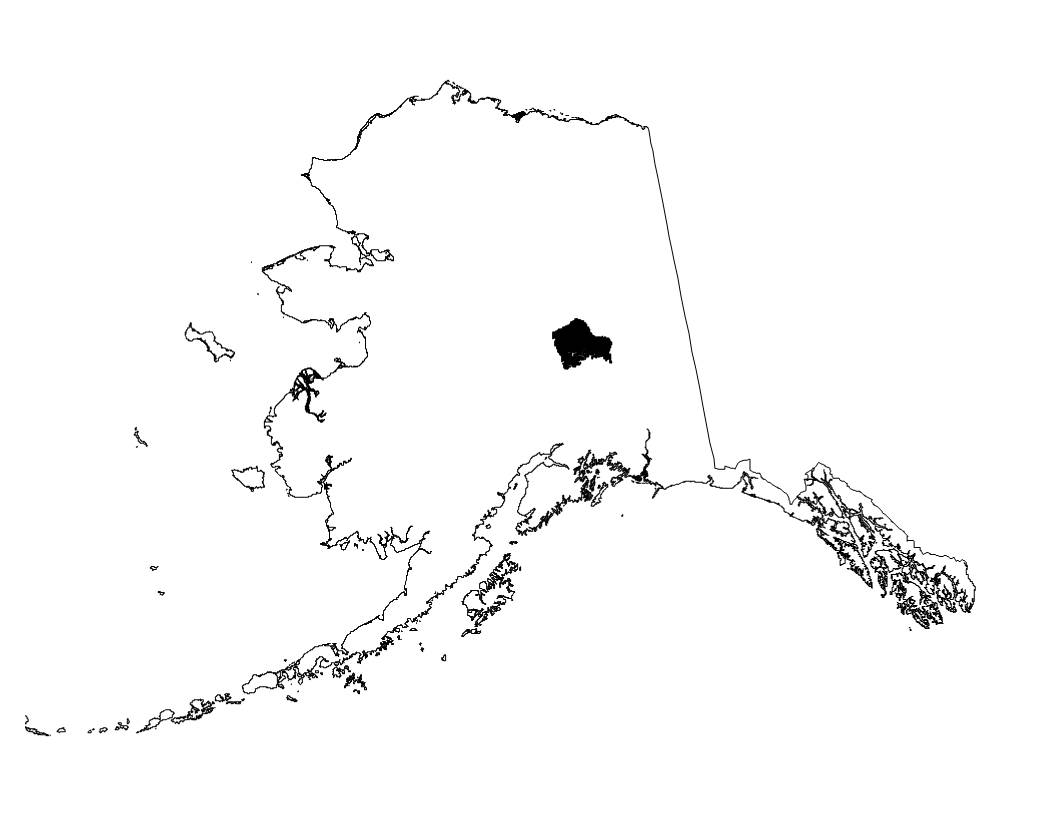
\includegraphics[width=6.3cm]{figure/mooseSurvey20A.jpg}  &
	
		\begin{itemize}
			\item Moose Survey
			\item South of Fairbanks
			\item $\sim$ 4500 mi$^2$
		\end{itemize}

	\end{tabular}

\end{frame}

%-------------------------------------------------------------------------------
%                        Spatial Sampling
%-------------------------------------------------------------------------------

\subsection{Spatial Sampling}
\begin{frame} 
     
	\begin{tabular} {p{2.7cm} p{4cm} p{2.7cm}}

		\begin{tabular} {p{2.7cm}}
			Total Area \\
			\vspace{.2cm} \cbl{SRS} \\
			\vspace{-.2cm} \begin{itemize}
				\item \small{$\hat{\tau} = 11535$}
				\item $\textrm{se}(\hat{\tau}) = 985$
			\end{itemize} \\
			\vspace{-.2cm} \cgr{FPBK} \\
			\vspace{-.2cm} \begin{itemize}
				\item \small{$\hat{\tau} = 11327$}
				\item $\textrm{se}(\hat{\tau}) = 978$
			\end{itemize} \\

		\end{tabular} &

		\vspace{-2cm} 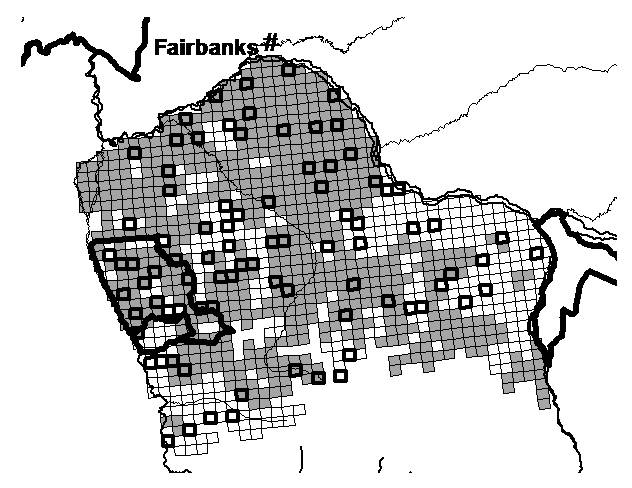
\includegraphics[width=4.3cm]{figure/MooseSurvey20APlots.jpg}  &
	
		\begin{tabular} {p{2.7cm}}
			Small Area \\
			\vspace{.2cm} \cbl{SRS(n=17)} \\
			\vspace{-.2cm} \begin{itemize}
				\item \small{$\hat{\tau} = 1535$}
				\item $\textrm{se}(\hat{\tau}) = 227$
			\end{itemize} \\
			\vspace{-.2cm} \cgr{FPBK} \\
			\vspace{-.2cm} \begin{itemize}
				\item \small{$\hat{\tau} = 1437$}
				\item $\textrm{se}(\hat{\tau}) = 153$
			\end{itemize} \\

		\end{tabular}

	\end{tabular}

\end{frame}


\end{document}
